\documentclass[../main.tex]{subfiles}
\hbadness=1000000
\vbadness=1000000

\begin{document}
\section{Results}
\subsection{Synchronization states in the Kuramoto motifs}
In this section, we present the synchronization states of the two motifs when each node or element is represented by a Kuramoto oscillator.
As we have previously discussed, this preliminary study helped us to understand the behavior of the motifs when they correspond to a network of coupled populations.
We have systematically examined the fixed point solutions associated with these motifs, considering the impact of connection delay (uniform across all connections) and introducing a detuning factor, which represents a positive or negative disparity in the intrinsic frequency of one oscillator.
This additional parameter was incorporated to align with our objective of identifying optimal conditions for enhancing communication between populations. Previous observations have indicated that even a minor mismatch in the intrinsic frequencies of the emitting oscillator serves to amplify communication effectiveness \citep{kirst_dynamic_2016,pariz_high_2018,pariz_transmission_2021}.

\subsubsection{V-motif}
Although we have already introduced the synchronization states of the V-motif in the introduction section, we will now also examine the situations in which the connections projected onto the relay element differ from the rest.
That is, $K_{12} = K_{32} \neq K_{21} = K_{23}$, and similarly when the frequency mismatch is applied to one of the external oscillators (1 by default) and the relay oscillator (2).

In the first case, shown in Figure \ref{fig:vmotif_omega0}, it can be observed that as the projections onto the relay oscillator become stronger, the size of the regions of instability are reduced.
At the same time, the effect of frequency mismatch decreases, and thus synchronization at zero time is maintained for the same values of this parameter.
In other words, the synchronization states at or near zero-lag between oscillators 1 and 3, observed at both low and high delays, and the anti-phase states between oscillators 1 and 2 at intermediate delays, exhibit increased robustness with heightened intensity in the projections onto oscillator 2.
\begin{figure}[!htb]
    \centering
    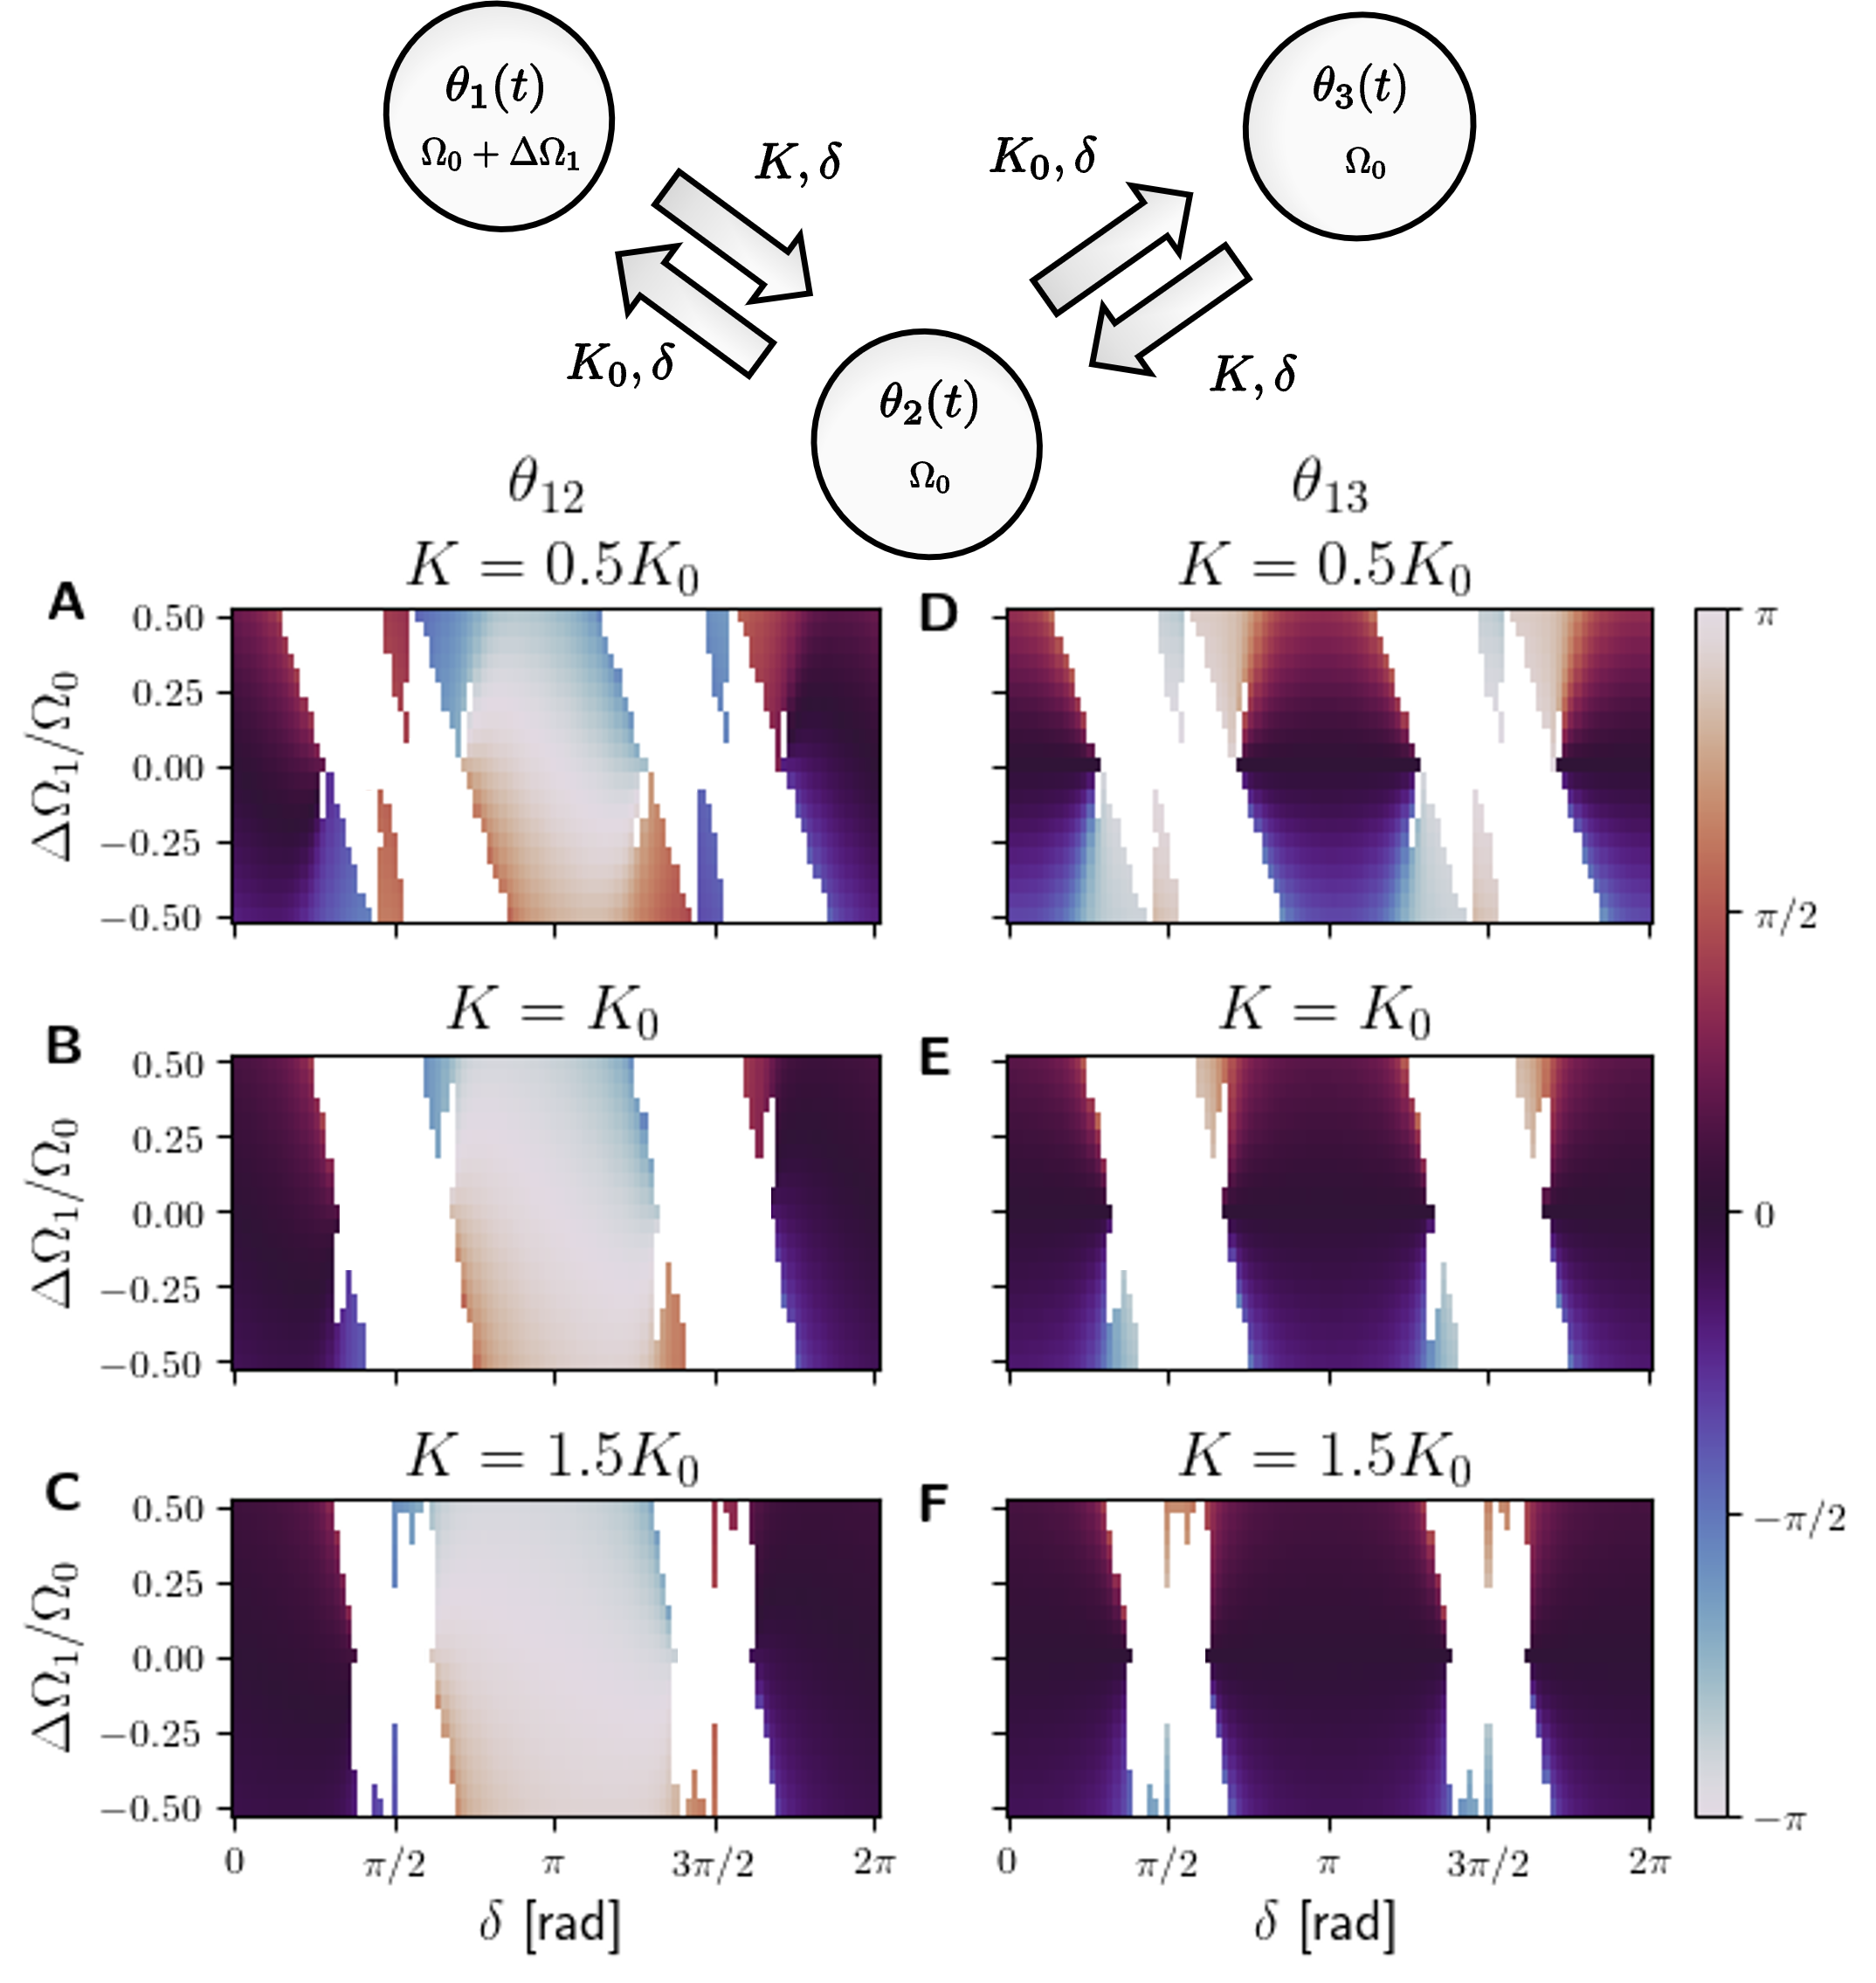
\includegraphics[width=\textwidth]{chapter2/figures/vmotif_different_omega_0_edited.png}
    \caption{\textbf{V-motif: phase-locked solutions}.
    Asymptotically stable fixed points of $\theta_{12}(t)$ (A-C) and $\theta_{13}(t)$ (D-F) as a function of the delay in the connections and the frequency mismatch $\Delta\Omega_1$ applied in oscillator 1.
    From top to bottom: $K'=0.5K_0$, $K'=K_0$ and $K'=1.5K_0$.
    White regions indicate the region with unstable fixed points.}
    \label{fig:vmotif_omega0}
\end{figure}
In the second scenario, shown in Figure \ref{fig:vmotif_omega1}, when the frequency mismatch is applied to oscillator 2, as we already know, the system remains symmetric.
That is, the baseline states ($\Delta\Omega$ = 0) are preserved, regardless of the value of $\Delta\Omega$. 
This only serves to shift the boundaries of the instability region.
Therefore, in this case, the coupling constants $K_{12}$ and $K_{32}$, as they increase, only play the role of reducing these regions of instability for the solutions.
\begin{figure}[!htb]
    \centering
    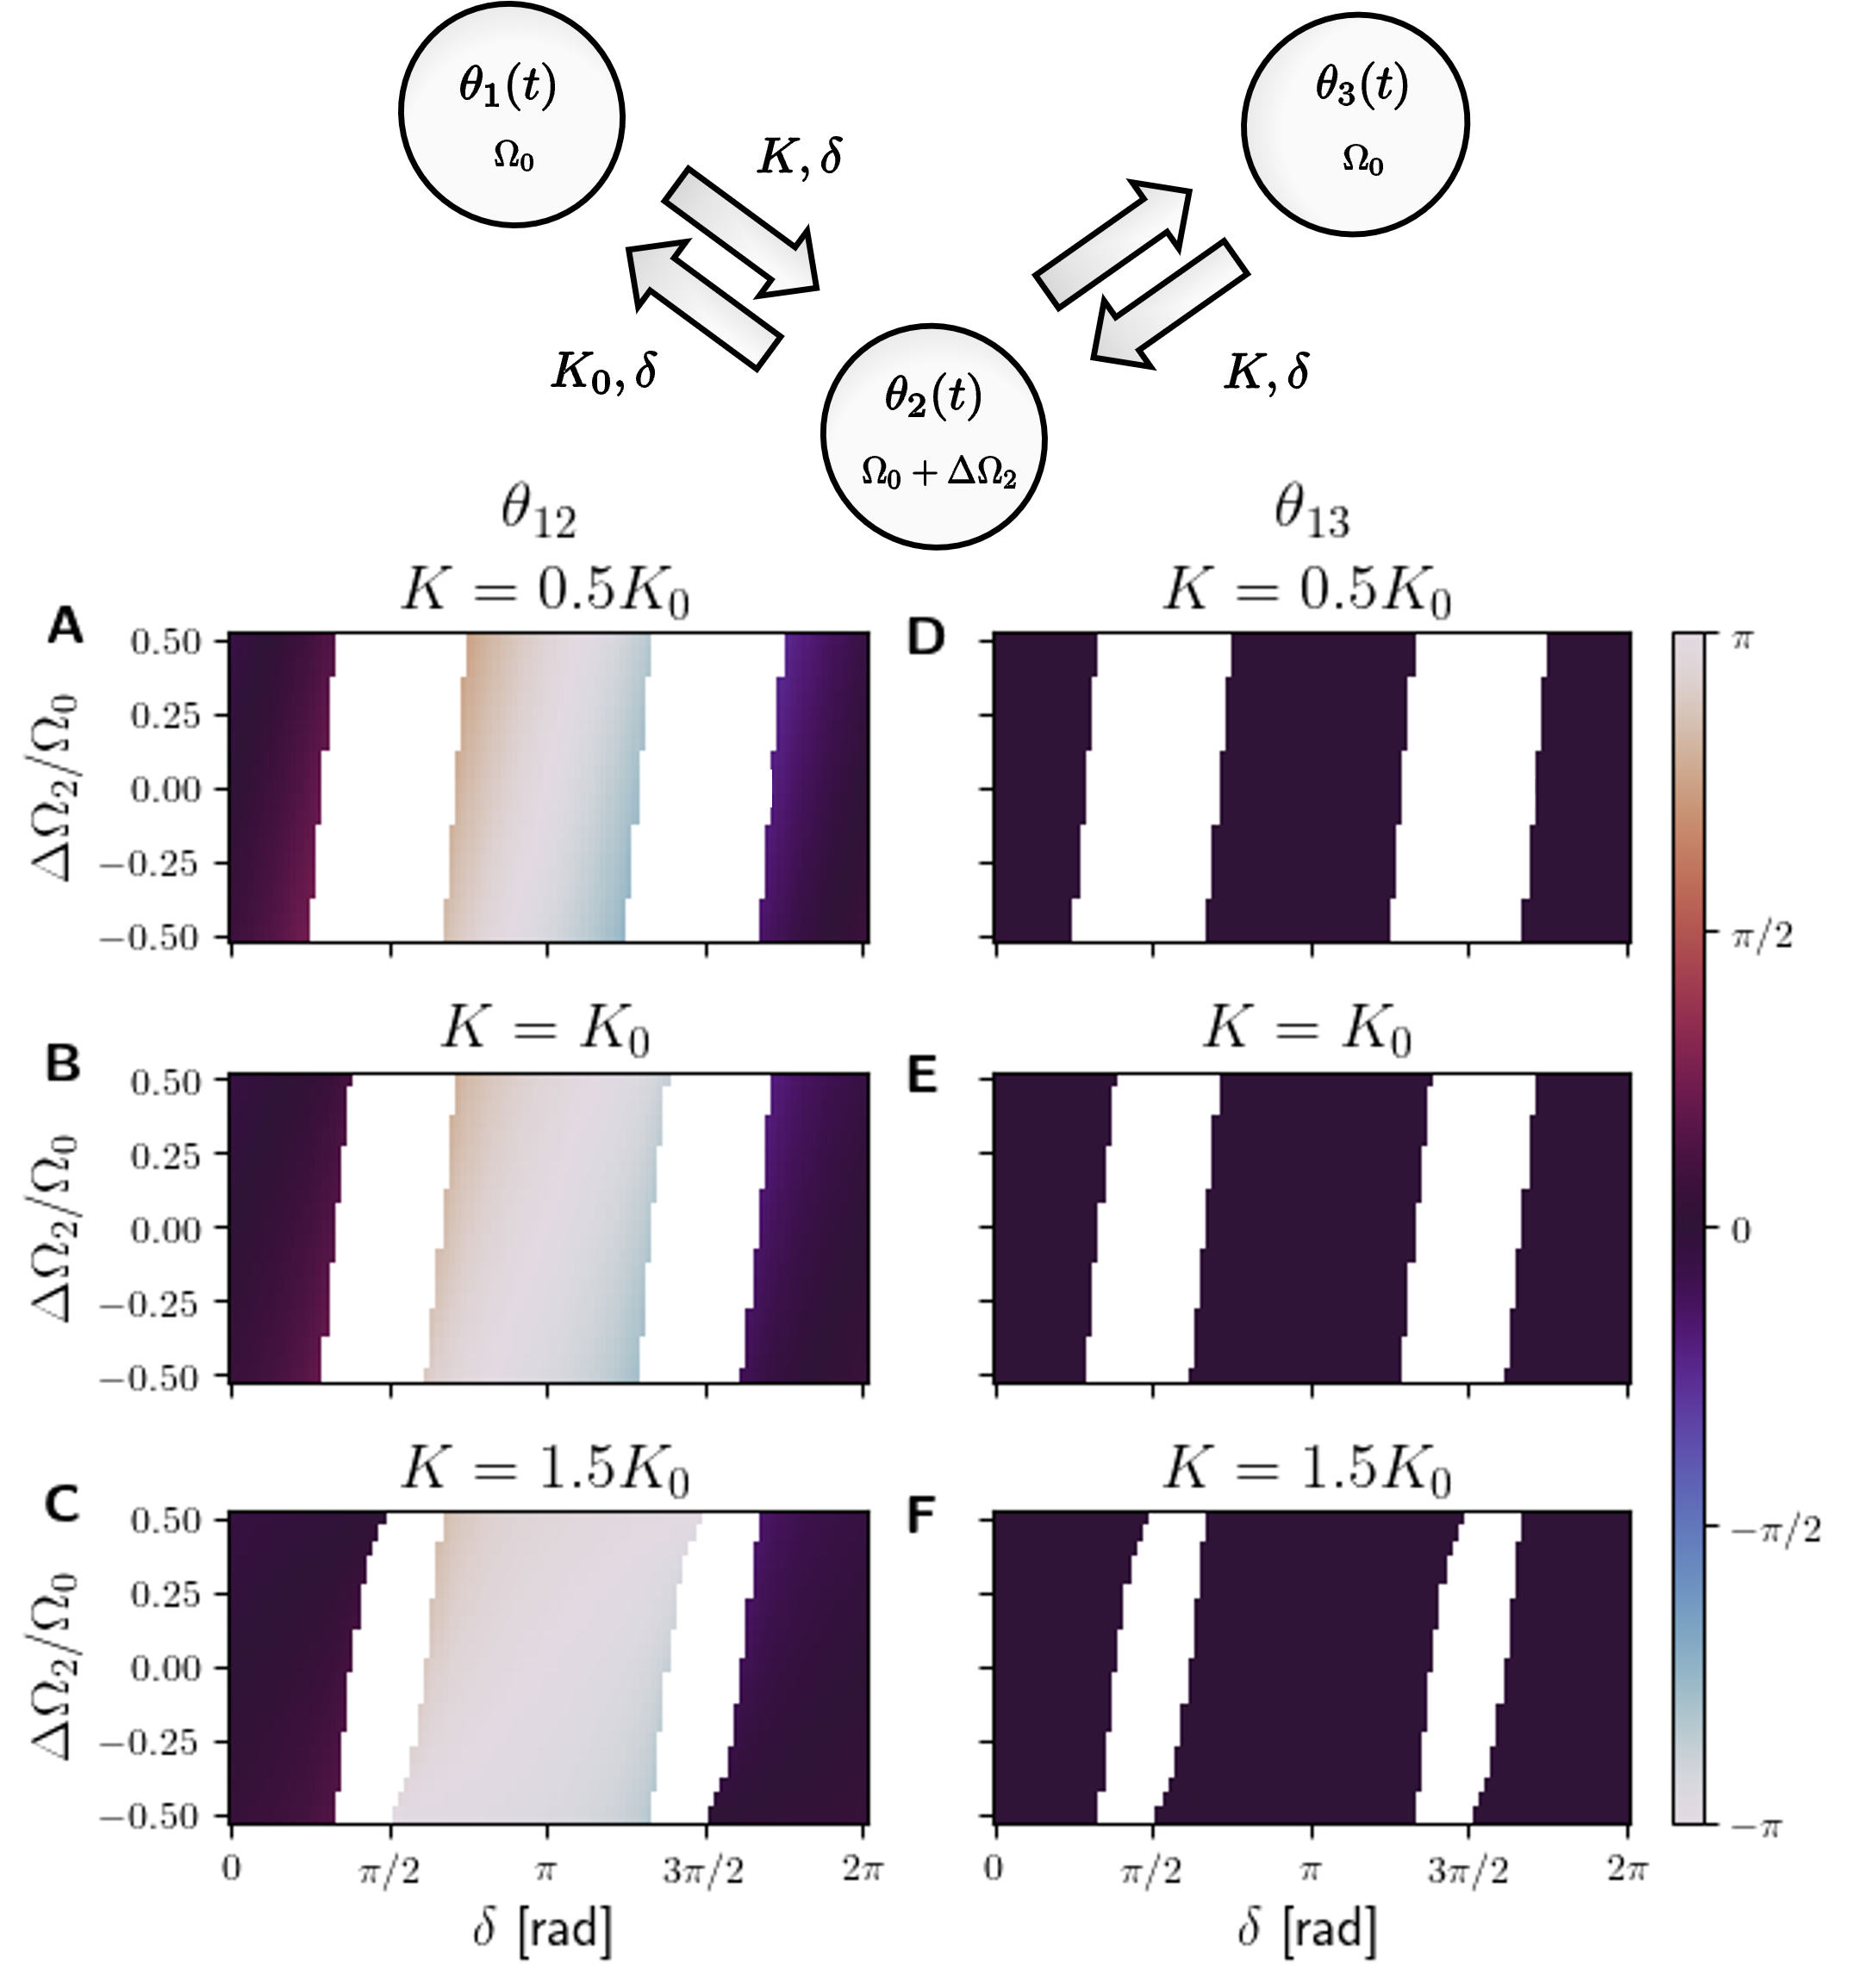
\includegraphics[width=\textwidth]{chapter2/figures/vmotif_different_omega_1_edited.png}
    \caption{\textbf{V-motif: phase-locked solutions}.
    Asymptotically stable fixed points of $\theta_{12}(t)$ (A, B, and C) and $\theta_{13}(t)$ (D, E, and F) as a function of the delay in the connections and the frequency mismatch $\Delta\Omega_2$ applied in oscillator 2.
    From top to bottom: $K'=0.5K_0$, $K'=K_0$ and $K'=1.5K_0$.
    White regions indicate the region with unstable fixed points.}
    \label{fig:vmotif_omega1}
\end{figure}
\clearpage
\subsubsection{C-motif}
The effect of adding the cortico-cortical connections, \textit{i.e.}, the connection between the outer oscillators $1$ and $3$, is shown in Figure \ref{fig:cmotif_bistability}.
In A and B, it can be observed the synchronization states as a function of the phase shift $\delta$ and the coupling constant $K' = K_{13} = K_{31}$.
In this scenario, as these connections increase, the stable region that appears for intermediate delays, $\theta_{12}$ around antiphase, gradually disappears while the bistability (the green region) emerges.
For $\delta=\pi$ and $K'= 0.5K_0$, a bifurcation occurs where the system transitions from stable to bistable (Figure \ref{fig:cmotif_bistability} C).
From this point on, for intermediate delay values, there is no longer a stable regime.
Another interesting bifurcation occurs when $K'=K_0$. 
For this specific point, no unstable solution exists. The stable solution corresponds to all three oscillators in phase, $\theta_{12}=\theta_{13}$, when $\delta \in [0,\pi/2) \cap [3\pi/2,2\pi)$, while the bistable solution $|\theta_{12}| = |\theta_{13}| \neq 0$ when $\delta \in [\pi/2, 3\pi/2)$.
From here, as $K'$ increases, regions of instability reappear, and another critical point appears at $K'=1.75K_0$, where the system transitions from a bistable to an unstable region, at $\delta = 3\pi/4$ and $\delta = 5\pi/4$.

Therefore, the cortico-cortical connection plays a significant role in the stability of the system, especially in the region of intermediate delays.
Up to levels of $K'=0.5K_0$, we observe a reduction in the sizes of both unstable and stable regions for intermediate delays. Simultaneously, this leads to an expansion in the stable region sizes for both low and high delays, along with an increase in the size of the bistable region.
From this point to $K'=K_0$, the region expands until it disappears.
At this point, the system is symmetric, meaning that all frequencies, delays, and constant couplings are equal to each other.
As $K'$ increases, the number of stable states decreases, while the number of unstable states increases. When $K'=1.75K_0$, new unstable states emerge in pursuit of the bistable states.
\begin{figure}[htpb]
    \centering
    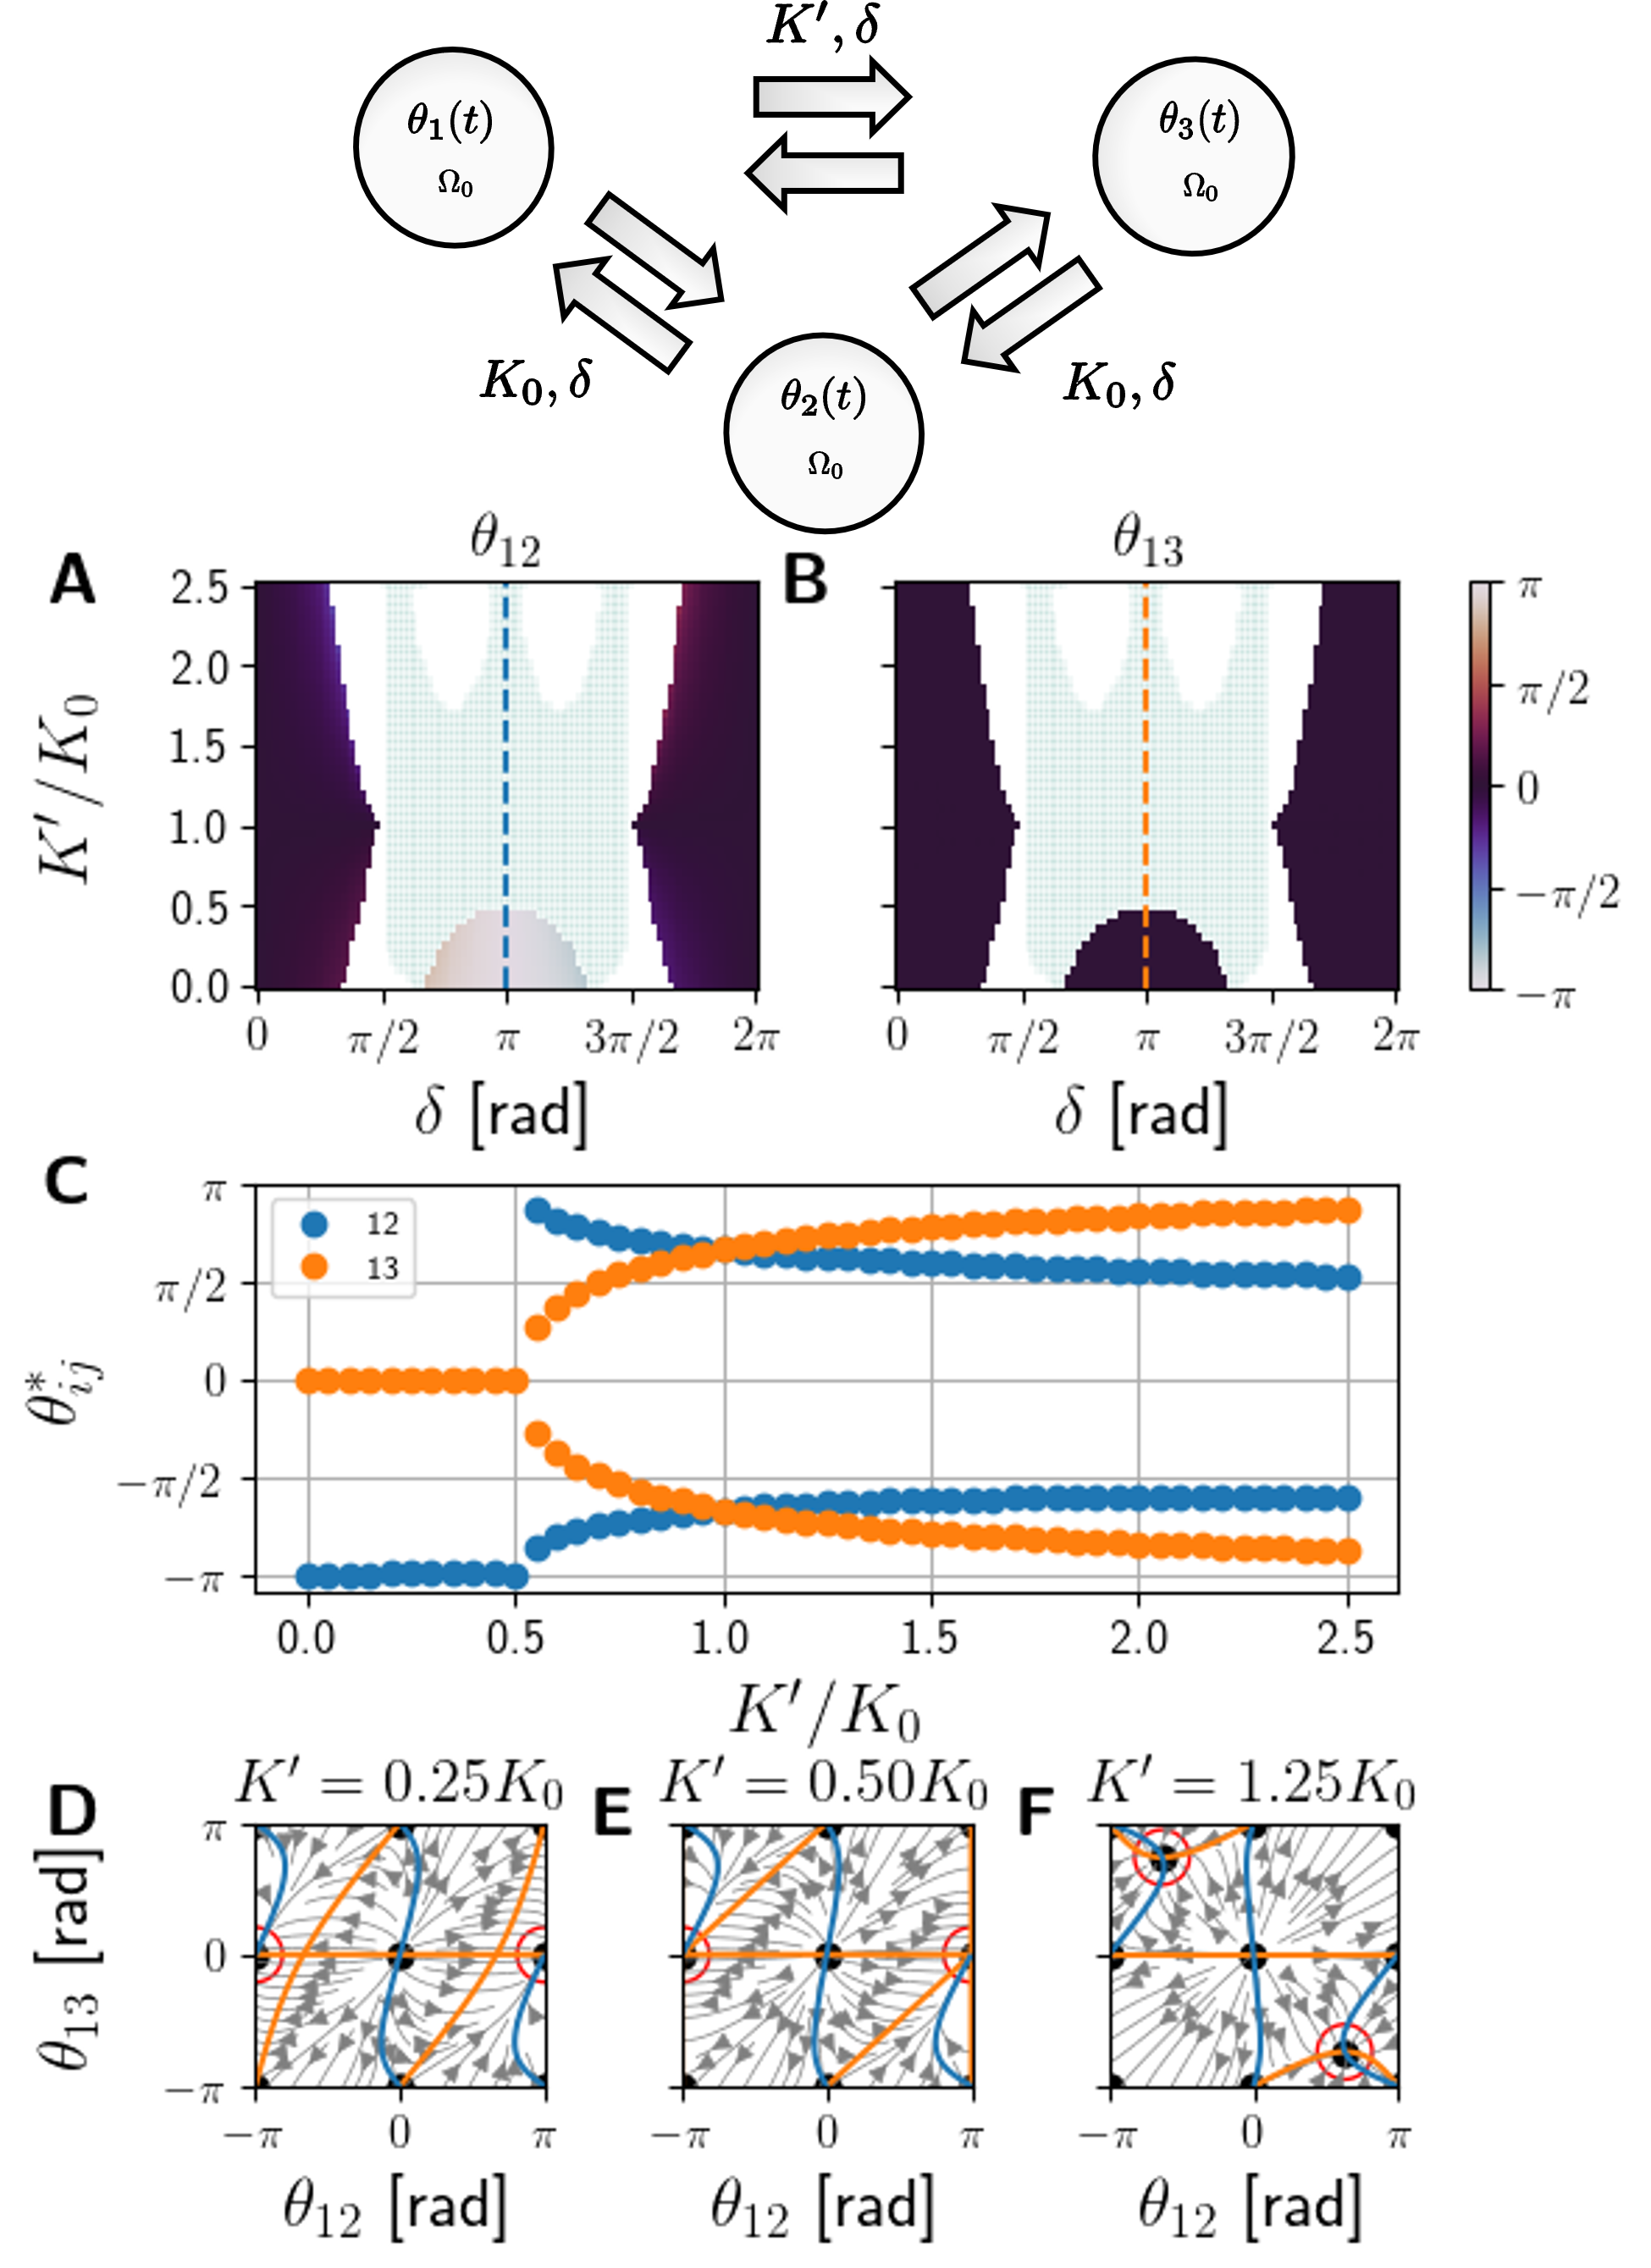
\includegraphics[width=0.9\textwidth]{chapter2/figures/cmotif_different_coupling_edited.png}
    \caption{\textbf{C-motif: emergence of bistability}. 
    Panels A and B indicate the phase differences $\theta_{12}$ and $\theta_{13}$, respectively.
    White regions indicate unstable solutions and green regions indicate bistability solutions.
    Blue and orange dashed lines refer to the values of $\theta_{12}$ and $\theta_{13}$, respectively, shown in C, where the bistable solution is depicted for $\delta = \pi$.
    D, E, and F show the corresponding phase diagram for $K'/K_0 = 0.25, 0.50$, and $0,75$, respectively.
    Blue and orange lines are the null-clines given by $\dot{\theta}_{12} = 0$ and $\dot{\theta}_{13}=0$, respectively.
    Red circles indicate the stable fixed points.}
    \label{fig:cmotif_bistability}
\end{figure}
\begin{figure}[!htb]
    \centering
    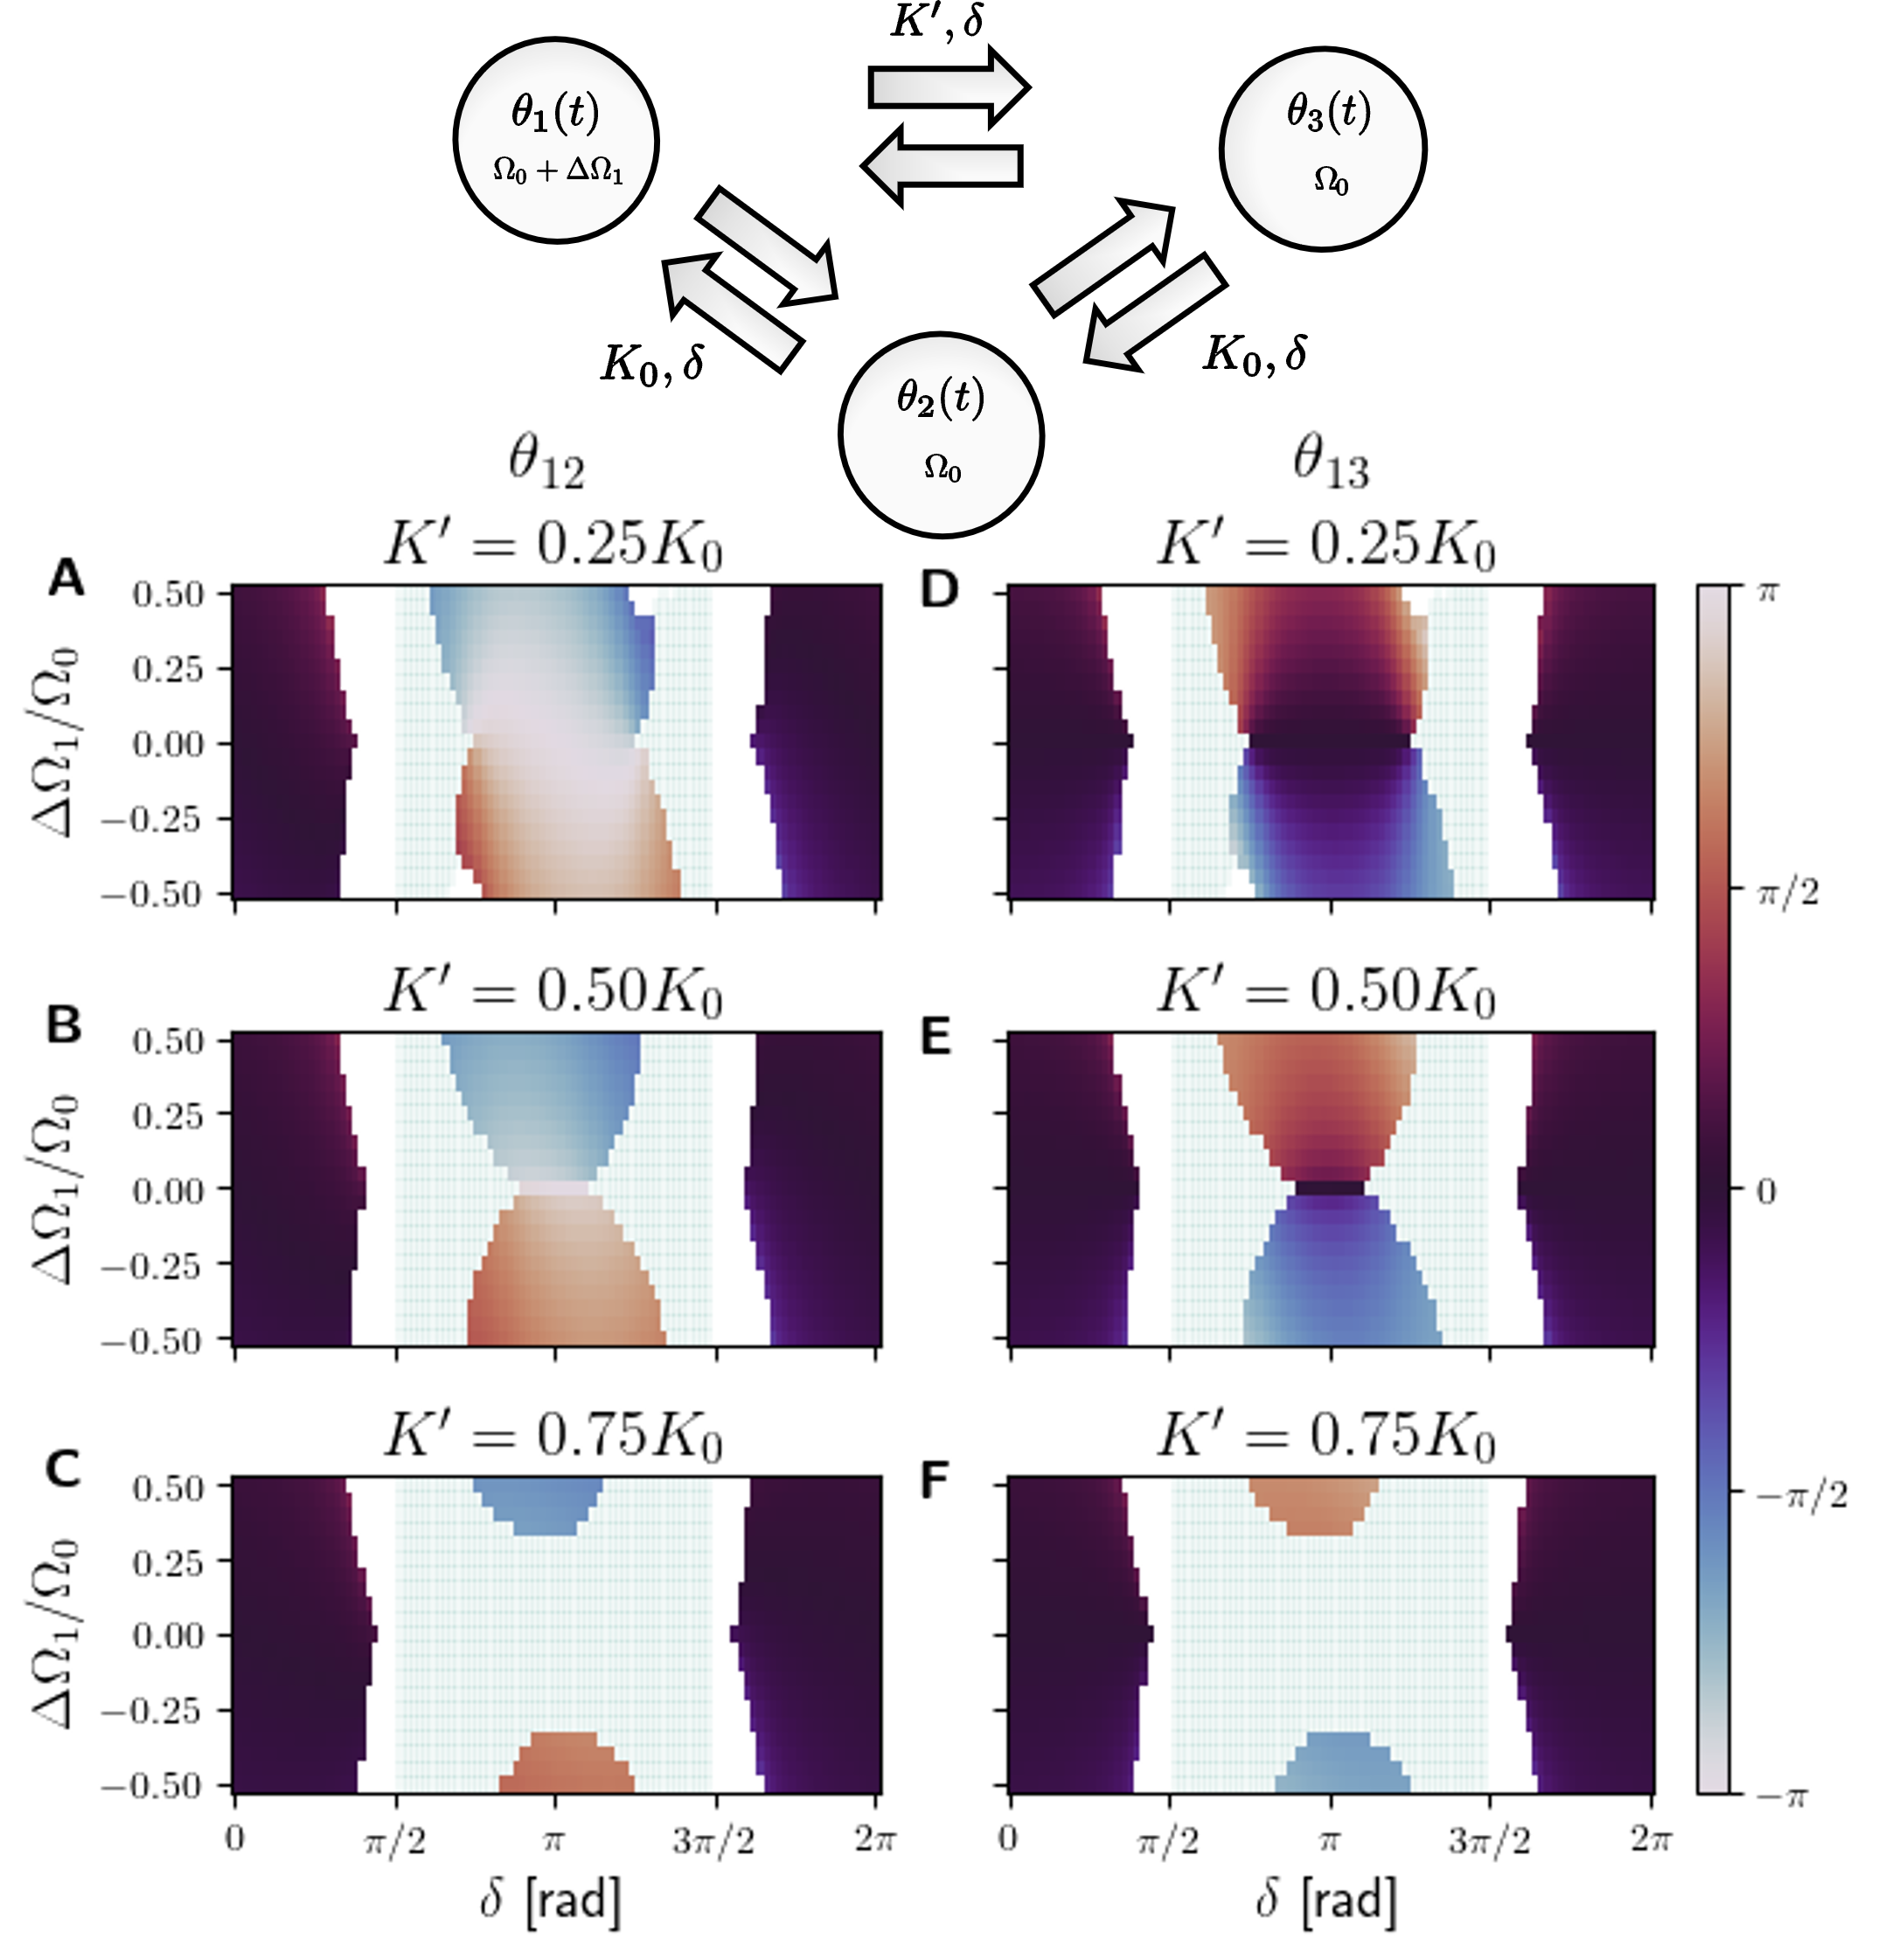
\includegraphics[width=\textwidth]{chapter2/figures/cmotif_different_omega_0_edited.png}
    \caption{\textbf{C-motif: phase-locked solutions}.
    Asymptotically stable fixed points of $\theta_{12}(t)$ (A, B and C) and $\theta_{13}(t)$ (D, E andF) as a function of the delay in the connections and the frequency mismatch $\Delta\Omega_1$ applied in oscillator 1.
    From top to bottom: $K'=0.25K_0$, $K'=0.50K_0$, and $K'=0.75K_0$.
    The white regions indicate the region with unstable fixed points.
    The green regions indicate where stable fixed points appear.}
    \label{fig:cmotif_omega1}
\end{figure}
We additionally investigated synchronization states for a specific cortico-cortical connection strength, examining how they vary as a function of both delay and frequency mismatch in oscillator 1 (Figure \ref{fig:cmotif_omega1}) and in the oscillator 2 (Figure \ref{fig:cmotif_omega2}).
The presence of this connection implies the emergence of a bistable solution in the system in the regions where this connection is small (Figures \ref{fig:cmotif_omega1} A and D, Figures \ref{fig:cmotif_omega2} A and D).
As this connection increases, the region of bistability grows as the stable region decreases.
In the case where the frequency mismatch is applied to oscillator 1, when $K' > 0.5K_0$, the anti-phase solution between 1 and 2 disappears (Figure \ref{fig:cmotif_omega1} C and F).
In contrast, when the frequency mismatch is applied to 2, and given that symmetry is still maintained, the intermediate region continues to exhibit the synchronization states of $\theta_{12} = \pi$ and $\theta_{13} = 0$. 
In general, as the cortico-cortical connection increases, it is necessary to apply a higher frequency mismatch (either more positive or more negative) to find stable solutions in the range of intermediate delays.
However, for low and high delays, the system is barely altered and we find stable solutions where the three oscillators are at zero phase.
In the range of intermediate delays, therefore, a competition between two dynamics occurs.
The dynamics of the V-motif tends to phase-lock oscillators 1 and 3, while the dynamics of the 2motif (1 and 3 connected) tend to put them in antiphase.
As a result of this competition, when $K' < 0.5K_0$, the dynamics of the V-motif dominates in the system, while when $K' = 0.5K_0$, bistability occurs as a consequence of the 2-motif dynamics having more influence on the overall dynamics.
\begin{figure}[!htb]
    \centering
    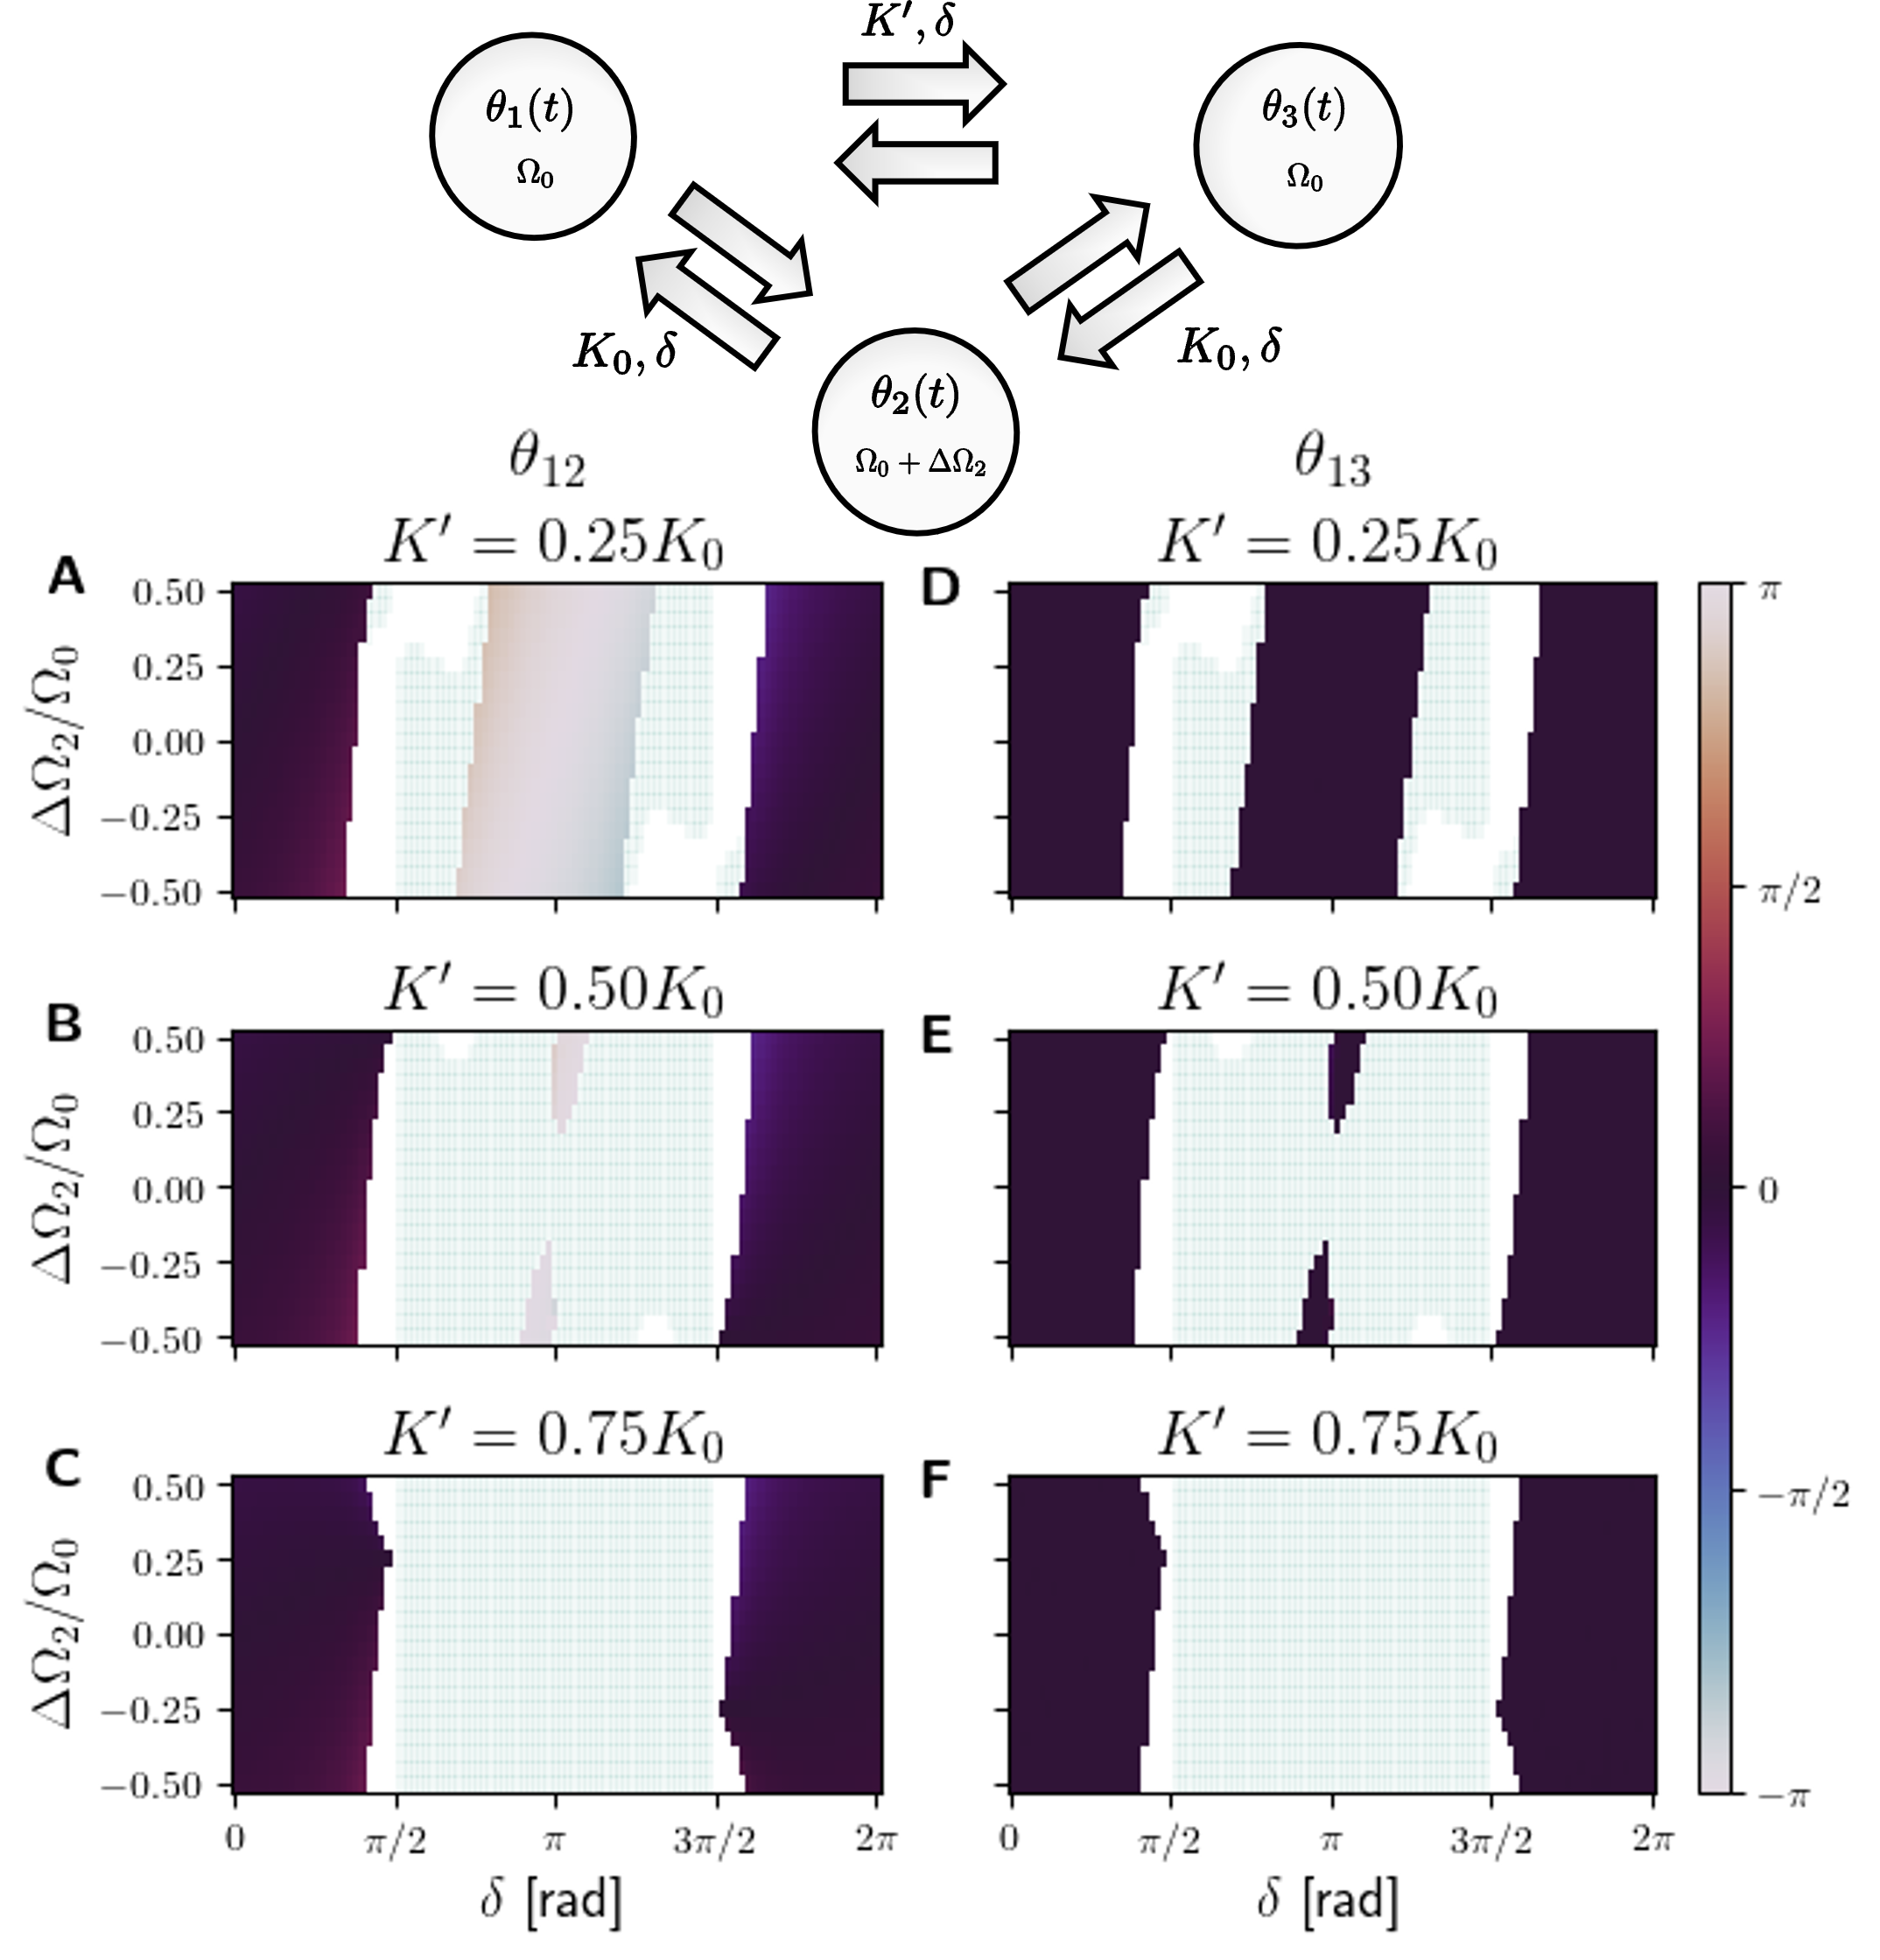
\includegraphics[width=\textwidth]{chapter2/figures/cmotif_different_omega_1_edited.png}
    \caption{\textbf{C-motif: phase-locked solutions}.
    Asymptotically stable fixed points of $\theta_{12}$ (A, B and C) and $\theta_{13}$ (D, E andF) as a function of the delay in the connections and the frequency mismatch $\Delta\Omega_1$ applied in oscillator 1.
    From top to bottom: $K'=0.25K_0$, $K'=0.50K_0$, and $K'=0.75K_0$.
    The white regions indicate the region with unstable fixed points.
    The green regions indicate where stable fixed points appear.}
    \label{fig:cmotif_omega2}
\end{figure}
\subsection{Synchronization and phase-locking in the V-motif}
% \textcolor{blue}{Aún hay que retocar un poco para enganchar lo anterior con esto.}
In the same way that we have analyzed the synchronization or phase-locking states of the Kuramoto motifs, we performed a similar analysis considering each node or element a balanced population of Hodgkin-Huxley neurons.
In this case, trhoughintensive numerical simulations we determined the fixed points of the system.
Considering the synchronization level of each node in the motif,  it can be treated as a simplified oscillator. 
This simplification allowed us to determine the firing rate (average number of spikes per unit of time) from the spikes, and subsequently associate a phase varaible to this oscillator.
Therefore, we considered the phase difference between two nodes as the median value of the distribution of phase differences obtained from the time series.
To accompany this measure, we used the phase-locking index to quantify the stability of the phase difference.
We also used it to define the stability regions in the same way as we did with the Kuramoto oscillators.

% \textit{We investigated the transmission of a signal from either population 1 or 2 to the remaining populations within the circuit.
% Our primary focus was to study the transmission process when there exists a frequency mismatch between the oscillation frequencies of the populations and when there is a non-zero transmission time between populations.
% In our analysis, two specific circuit configurations, namely the V-motif and the C-motif were considered.
% Initially, we present our findings for the V-motif, neglecting the cortico-cortical connections ($g_{13} = g_{31} = 0$ $\mu$S/cm$^2$).
% We assumed symmetric coupling strengths between populations, denoted as $g_{12} = g_{21} = g_{23} = g_{32}$.
% \textcolor{red}{(Results for asymmetric cases are provided in the supplementary material)}.
% It is important to note that each isolated neural population exhibits highly synchronized behavior, which is maintained even when they are coupled.}
Given our primary focus on investigating the transmission of information from either the outer population (1) or the relay population (2) to the remaining populations, we examined two identical scenarios when analyzing locking regions, as previously conducted.
In one scenario, the frequency mismatch was applied to population 1 (or equivalently, population 3), and in the other, it was applied to population 2.

By analyzing the phase-locking regions in the space parameter, $\tau$ and $\Delta I$, we typically observed the same three regions. bounded by two non-locked regions as observed with Kuramoto oscillators (panels A and E of Figure \ref{fig:vmotif_signal_1} and Figures \ref{a-fig:vmotif_locking_1}, \ref{a-fig:vmotif_phase_difference_1}, \ref{a-fig:vmotif_locking_2} and \ref{a-fig:vmotif_phase_difference_2} in Appendinx A).

The locking regions between populations 1 and 2, as well as between populations 1 and 3, are illustrated in the parameter space of $\Delta I$ versus $\tau$ in panel A (E) of Figure \ref{fig:vmotif_signal_1} when the detuning $\Delta I$ was applied to population 1, and in Figure \ref{fig:vmotif_signal_2} when it was applied to population 2.
As expected, the locking regions are slightly larger between populations 1 and 2 compared to populations 1 and 3, although both cases exhibit a high locking-phase index.
The phases in which the oscillations of populations 1 and 2 (1 and 3) locked are displayed in panels B (F) of Figures \ref{fig:vmotif_signal_1} and \ref{fig:vmotif_signal_2}.
In the absence of detuning ($\Delta I=0$), we observed zero-lag synchronization between populations 1 and 3.
In addition, for small and large delays (close to the oscillation period), populations 1 and 2 exhibit nearly in-phase behavior.
However, for intermediate delay values, antiphase dynamics was observed, as expected from the previous analysis with Kuramoto oscillators \citep{vicente_dynamical_2008,esfahani_zero-lag_2014,mirasso_anticipated_2017}.

% \textcolor{blue}{Dudoso de si mantener aqui los ejemplos o ponerlos en la sección de métodos donde puse los comentarios.} \textcolor{red}{a mi me parecen bien aquí}
Examples demonstrating the activity of the three populations and their firing rates are shown in Figure \ref{fig:vmotif_series_1}, panels A, B, and C, for different detuning values when the connection delay was fixed at 6 ms.
\begin{figure}[!htb]
 \centering
    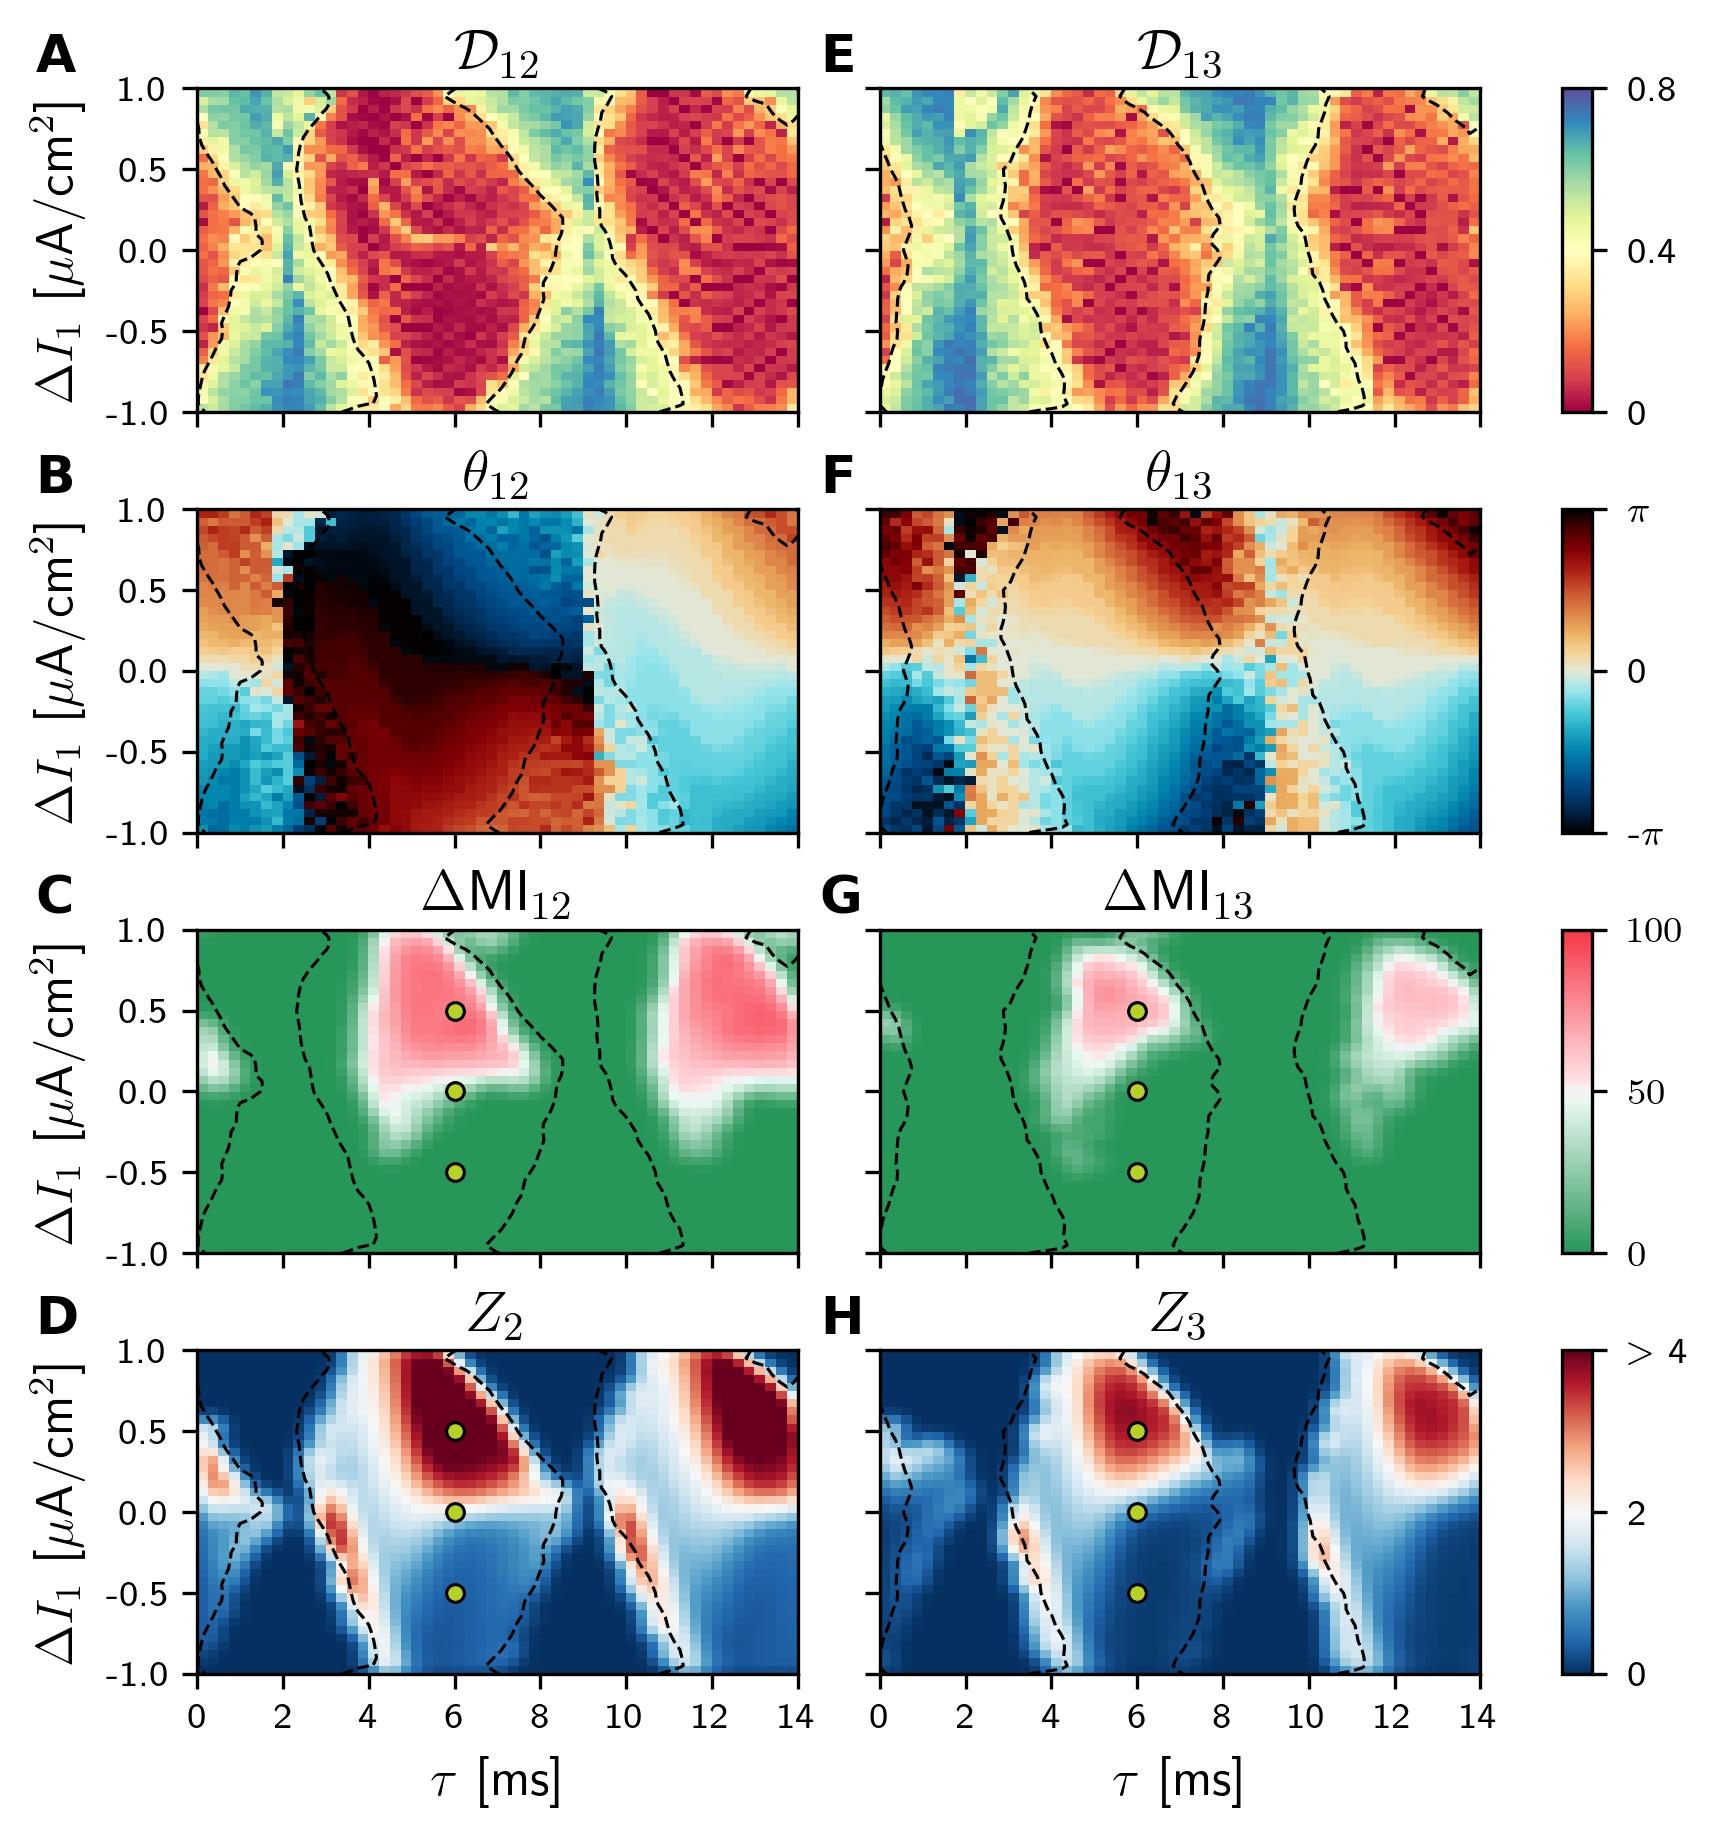
\includegraphics[width=\textwidth]{chapter2/figures/fig2}
    \caption{\textbf{V-motif: population 1 as sender}.
    Phase-locking index $\mathcal{D}_{ij}$ (A and D).
    Phase difference $\theta_{ij}$ (B and E). Difference $\Delta$MI$_{ij}$ (C and F).
    Integral of the absolute value of the nPRC $Z_i$ (D and H).
    All of them as a function of the delay $\tau$ and the frequency mismatch $\Delta I$ in population 1.
    The yellow points indicate the values of $\Delta I$ (-0.5, 0.0, 0.5 $\mu$A/cm$^2$) and $\tau$ (6 ms) corresponding to the examples of temporal series and nPRCs depicted in Figure \ref{fig:vmotif_series_1}.}
    \label{fig:vmotif_signal_1}
\end{figure} 
In the presence of non-zero detuning ($\Delta I \ne 0$) and for small or large delays, the locking phase deviates from zero and becomes positive (delayed synchronization) for positive detuning, and negative (anticipated synchronization) for negative detuning.
It is important to mention that similar results to those depicted in Figure \ref{fig:vmotif_signal_1} were obtained when considering different coupling strength values (Appendinx A Figures \ref{a-fig:vmotif_locking_1} and \ref{a-fig:vmotif_locking_2}).

\subsection{Information transmission in the V-motif}
Depending on whether we analyzed the transmission of a slow modulation or a fast pulse chain, we employed different methodologies.
The effect of the slow modulation signal manifests as a modulation of the firing rate while keeping the oscillation frequency similar, whereas each pulse of the fast signal alters the duration of the ongoing oscillation cycle.
Consequently, these two effects occur at different time scales, and then different tools are required for their quantification.

\begin{figure}[!htb]
 \centering
    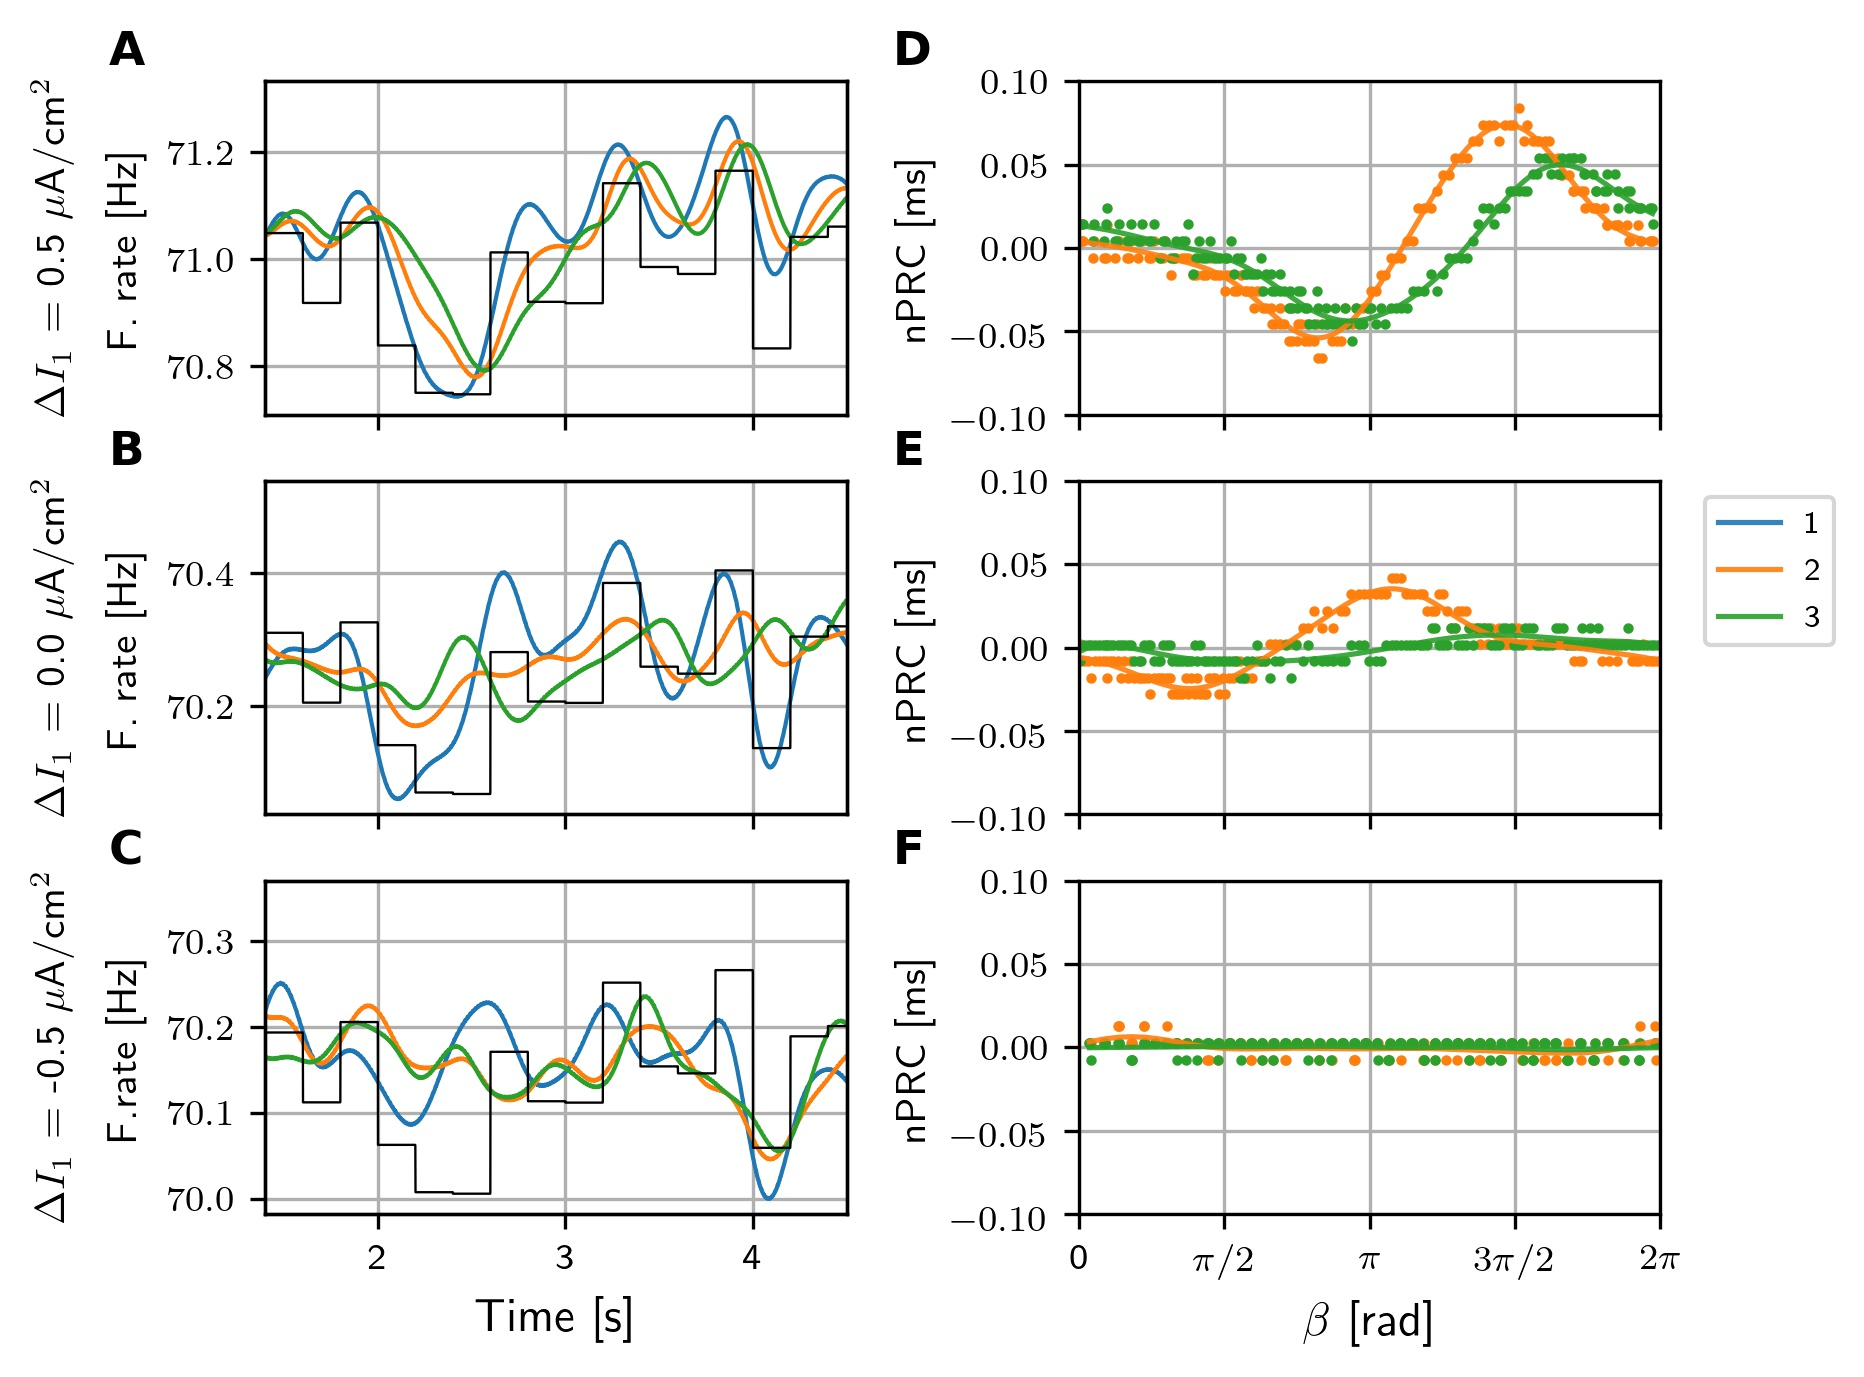
\includegraphics[width=\textwidth]{chapter2/figures/fig3}
    \caption{\textbf{V-motif}: Examples of firing rates of the three populations for different values of the frequency mismatch $\Delta I$ when a slow arbitrary signal (black line) is applied to population 1 (A, B, and C).
    Examples of non-local phase response curves of the receiving populations for the same different values of frequency mismatch $\Delta I$ when a fast pulsating signal is applied in population 1 (D, E, and F).
    Delay $\tau$ = 6 ms in all cases.}
    \label{fig:vmotif_series_1}
\end{figure}
For the case of slow modulation, we used two different measurements: the zero-lag cross-covariance (ZLC) between the firing rate of the receiving population and the injected signal, and the difference $\Delta$MI$_{ij}$ computed from the time-delayed mutual information between the firing rates of the sender and receiver populations.
Figure \ref{fig:vmotif_signal_1}, panels C and G, show the results for $\Delta$MI$_{ij}$ when population 1 (cortical area) acts as the sender and a slow modulation signal is injected (the phase-locking limits from panels A and E are also included here with dashed lines). 
We have also studied asymmetric scenarios where $g_{12}\neq g_{21}$ and $g_{23} \neq g_{32}$.
The correspondent plots of these cases can be found in Appendinx A Figure \ref{a-fig:vmotif_dmi_1}, as well as the results of ZLC measurements in Figure \ref{a-fig:vmotif_cov_1}.

Generally, regions with high values of $\Delta$MI$_{ij}$ in Figure \ref{fig:vmotif_signal_1} and high values of ZLC exhibit qualitative agreement, despite quantifying different properties.
Covariance quantifies the similarity in activity between two populations, whereas $\Delta$MI$_{ij}$ provides insight into the strength (absolute value) and directionality (sign) of the transmission.
Nonetheless, we noted a heightened correlation between these two quantities as the phase-locking index approaches zero, indicating a state of perfect locking (Appendinx A Figures \ref{a-fig:vmotif_histogram_1_100}, \ref{a-fig:vmotif_corr_1} and \ref{a-fig:vmotif_corr_2}).
Furthermore, we found that in cases where the values of $\Delta$MI$_{ij}$ and cross-covariance are the highest, the phase-locking index is very close to zero, indicating a constant, well-defined phase relation.
This finding aligns well with the Communication Through Coherence hypothesis, which posits that a well-defined phase relation is essential for enhancing communication between neural populations \citep{fries_rhythms_2015}.

We found that the optimal approach to transmit a slow modulation signal from population 1 to 2 and then to 3 is by imposing a positive detuning $\Delta I$ in the sender population (Figure \ref{fig:vmotif_signal_1}, panels C and G).
For negative values of the detuning, the transmission is significantly weakened.
These findings are consistent with previous results \cite{pariz_high_2018,pariz_transmission_2021}.
The yellow points in Figure \ref{fig:vmotif_signal_1}, panels C and G, correspond to the selected values of the detuning $\Delta I$, which characterize the temporal series presented in Figure \ref{fig:vmotif_series_1}, panels A, B, and C, for a delay of $\tau = 6$ ms.
In cases where the points fall within the red region in Figure \ref{fig:vmotif_series_1}, the firing rate of the receiver populations closely follows the injected signal.
In contrast, those outside the red regions do not exhibit this behavior.
Higher $\Delta$MI$_{1,2}$ values indicate more similarity between the modulation effect in the firing rates of the two populations, occurring at a much longer time scale than that of the gamma oscillations.
\begin{figure}[!htb]
 \centering
    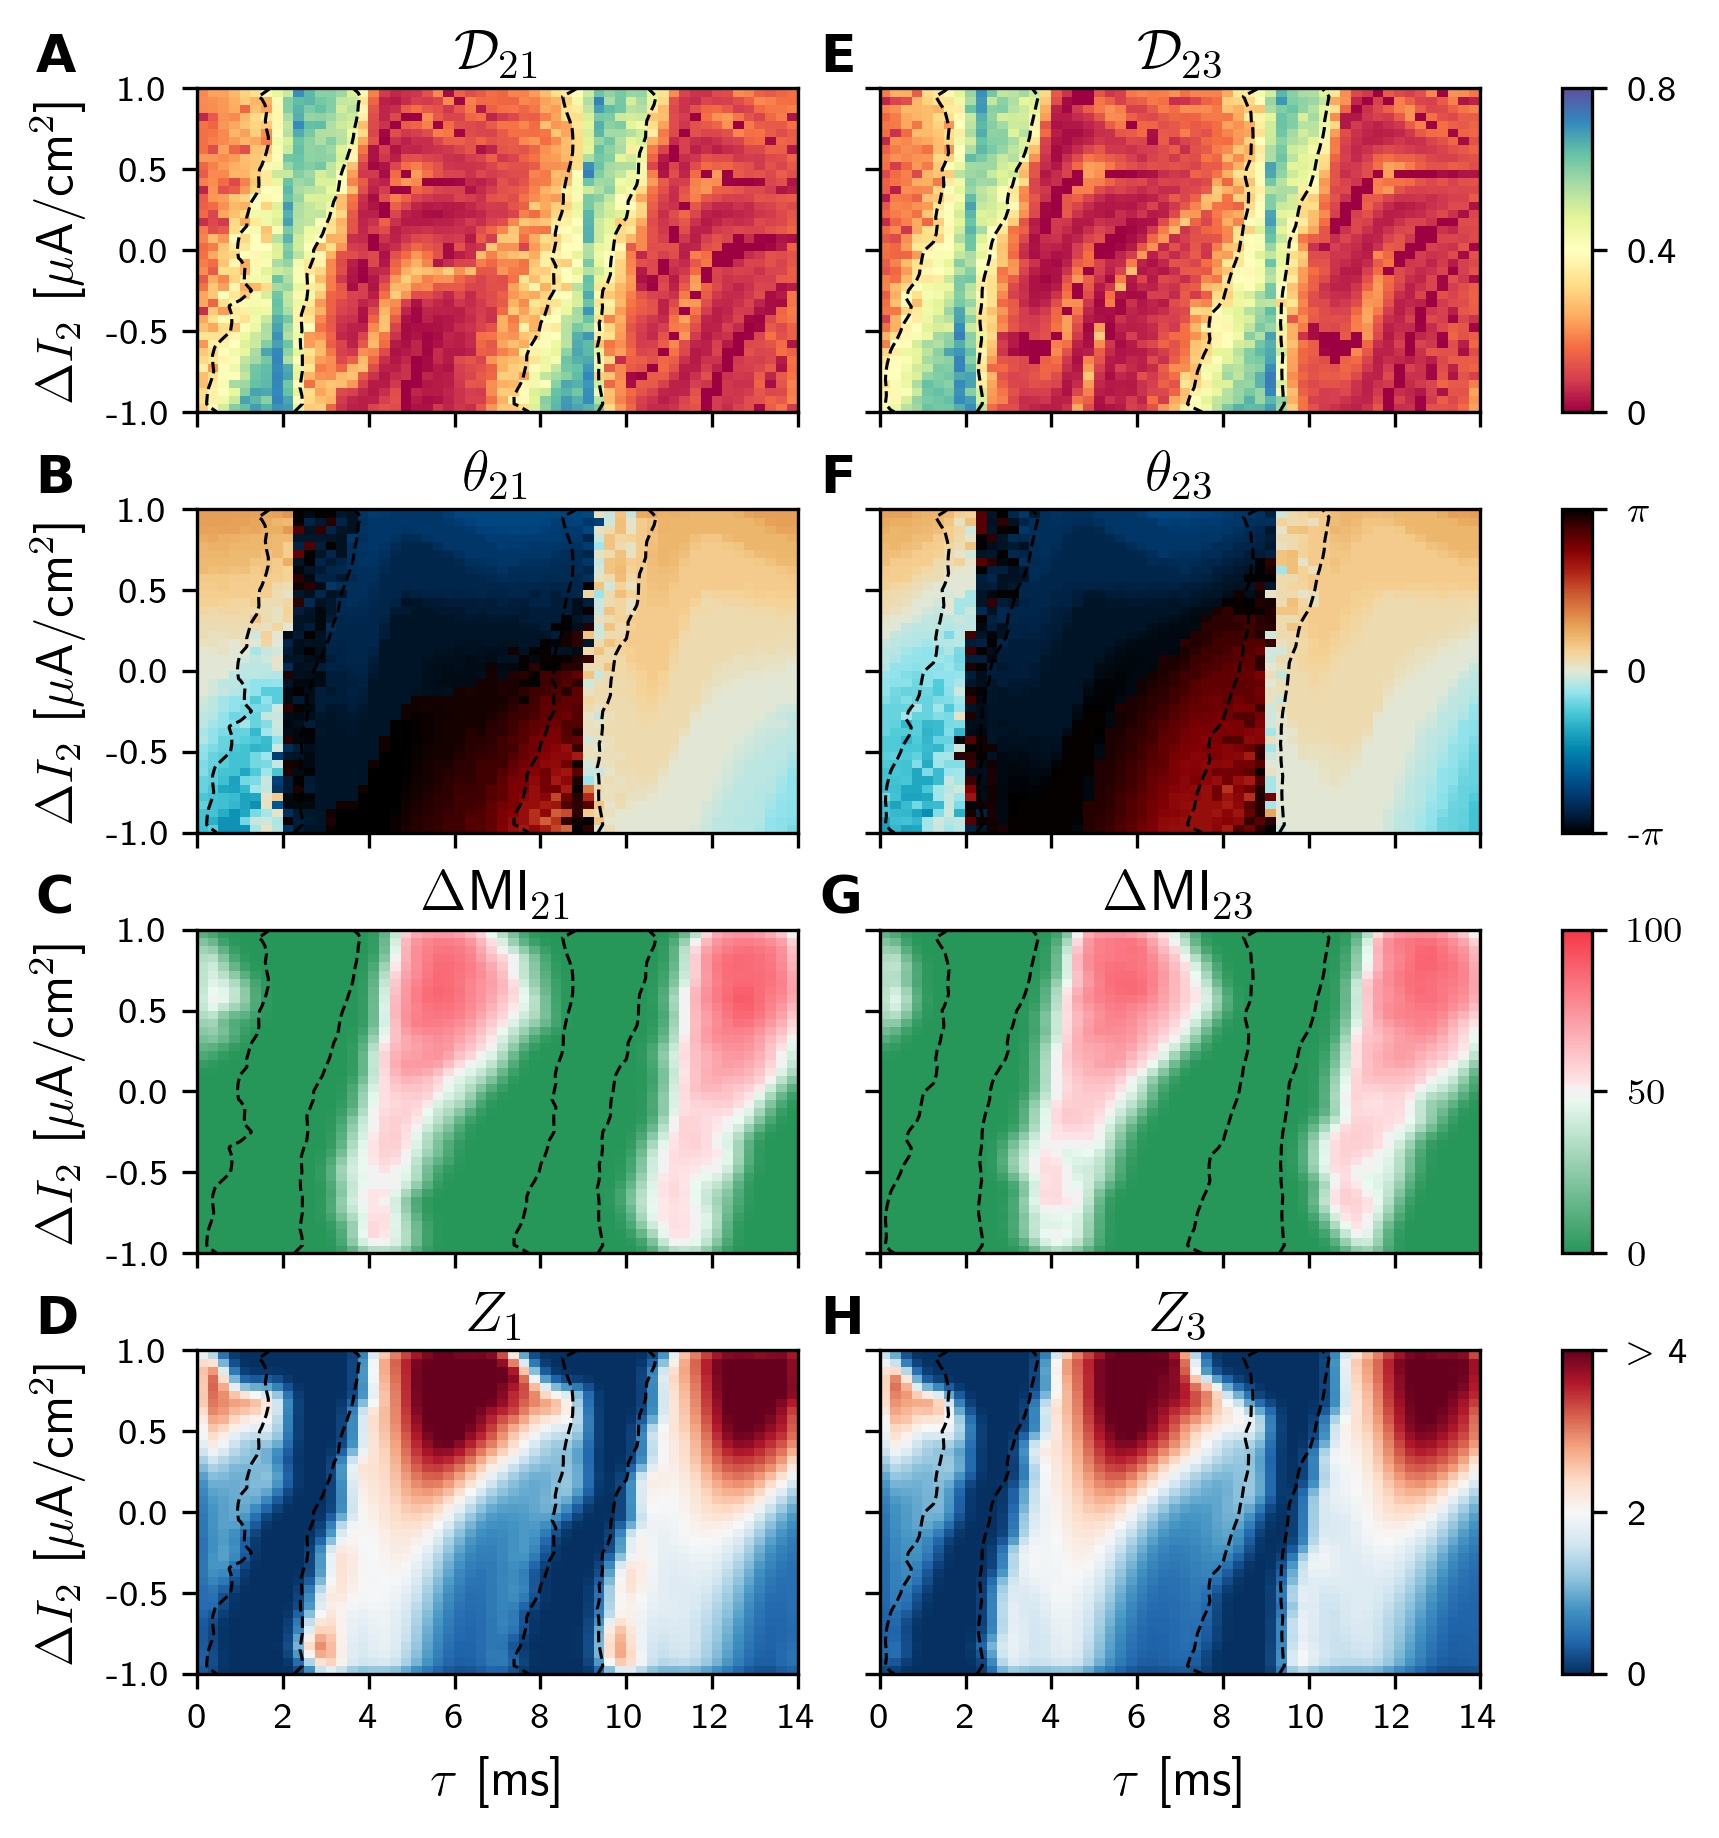
\includegraphics[width=\textwidth]{chapter2/figures/fig4}
    \caption{\textbf{V-motif: population 2 as sender}.
    Phase-locking index $\mathcal{D}_{ij}$ (A and D).
    Phase difference $\theta_{ij}$ (B and E).
    Difference $\Delta$MI$_{ij}$ (C and F).
    Integral of the absolute value of the nPRC $Z_i$ (D and H).
    All of them as a function of the delay $\tau$ and the detuning $\Delta I$ in population 2.}
    \label{fig:vmotif_signal_2}
\end{figure}
It is worth noting that although the time evolution of the firing rates may appear similar for some cases of negative detuning, none of them accurately track the injected signal.

Consistent findings emerged when a rapidly pulsating signal was injected, as opposed to the slow modulation signal.
In this case, we computed the integral of the absolute value of the non-local phase response curve (nPRC) of the receiving populations.
Figure \ref{fig:vmotif_signal_1}, panels D and H, display the outcomes where it can be observed that the regions demonstrating better transmission align quite well with those observed in the slow modulation case.
For these colormaps, we set $Z_i = 0$ when the resultant dynamics does not exhibit a PRC shape-like pattern, assuming that there is no signal transmission.
In addition, Figure \ref{fig:vmotif_signal_1}, panels D, E, and F, illustrate examples of the nPRCs of the receiving populations (orange and green) for specific parameter values indicated with yellow points in Figure \ref{fig:vmotif_signal_1}, panels G and H.
Analytical expressions for fitting cannot be obtained for points lying outside the locking areas.
In general, we observed that the information transmission, whether rate (slow) or spike coding (fast), changes with the strength $g$, improves as $g$ increases (Appendinx A Figures \ref{a-fig:vmotif_prc_1}).

The situation undergoes a drastic change when population 2 (the thalamus in our cortico-thalamic-cortical assumption) acts as the sender.
Notably, the system maintains symmetry even in the presence of a detuning.
Transmission of a slow signal to populations 1 and 3 is equivalent, as demonstrated in Figure \ref{fig:vmotif_signal_2}, panels C and G (asymmetric cases can be seen in Appendinx A Figure \ref{a-fig:vmotif_dmi_2} and  Figure \ref{a-fig:vmotif_cov_2} for the ZLC colormaps).
Furthermore, transmission is possible in this scenario even for negative values of the detuning, particularly for intermediate and long delays.
This result aligns with the case of two mutually-coupled neural populations reported in \citep{pariz_transmission_2021} and is a direct consequence of the system's symmetry.
However, we discovered that the signal transmission capability under these conditions is reduced as the cortico-thalamic synaptic strength increases.% (results not shown).

A similar behavior is observed when a fast random signal is injected, as depicted in Figure \ref{fig:vmotif_signal_2}, panels D and H, which illustrate the patterns of $Z_i$ (asymmetric cases in Appendinx A Figure \ref{a-fig:vmotif_prc_2}).

\subsection{Synchronization and phase-locking in the circular motif}
After introducing a cortico-cortical connection, the circuit adopts a ring topology.
Four different values of the synaptic strength $g'$ between the outer populations (= $g_{13}$ = $g_{31}$) were considered: 0.05$g_0$, 0.25$g_0$, 0.50$g_0$, and 0.75$g_0$, all weaker than the cortico-thalamic and thalamo-cortical connections.
The results presented in this section focus on two specific values: $g$ = 0.25$g_0$ (low) and $g$ = 0.75$g_0$ (high). 
% Results for the remaining $g'$ values can be found in the Appendix (\textbf{REFERNECIAS LAS FIGURAS}).
The strength of the thalamo-cortical and cortico-thalamic synapses remains constant at $g_0$.
\begin{figure}[!htb]
 \centering
    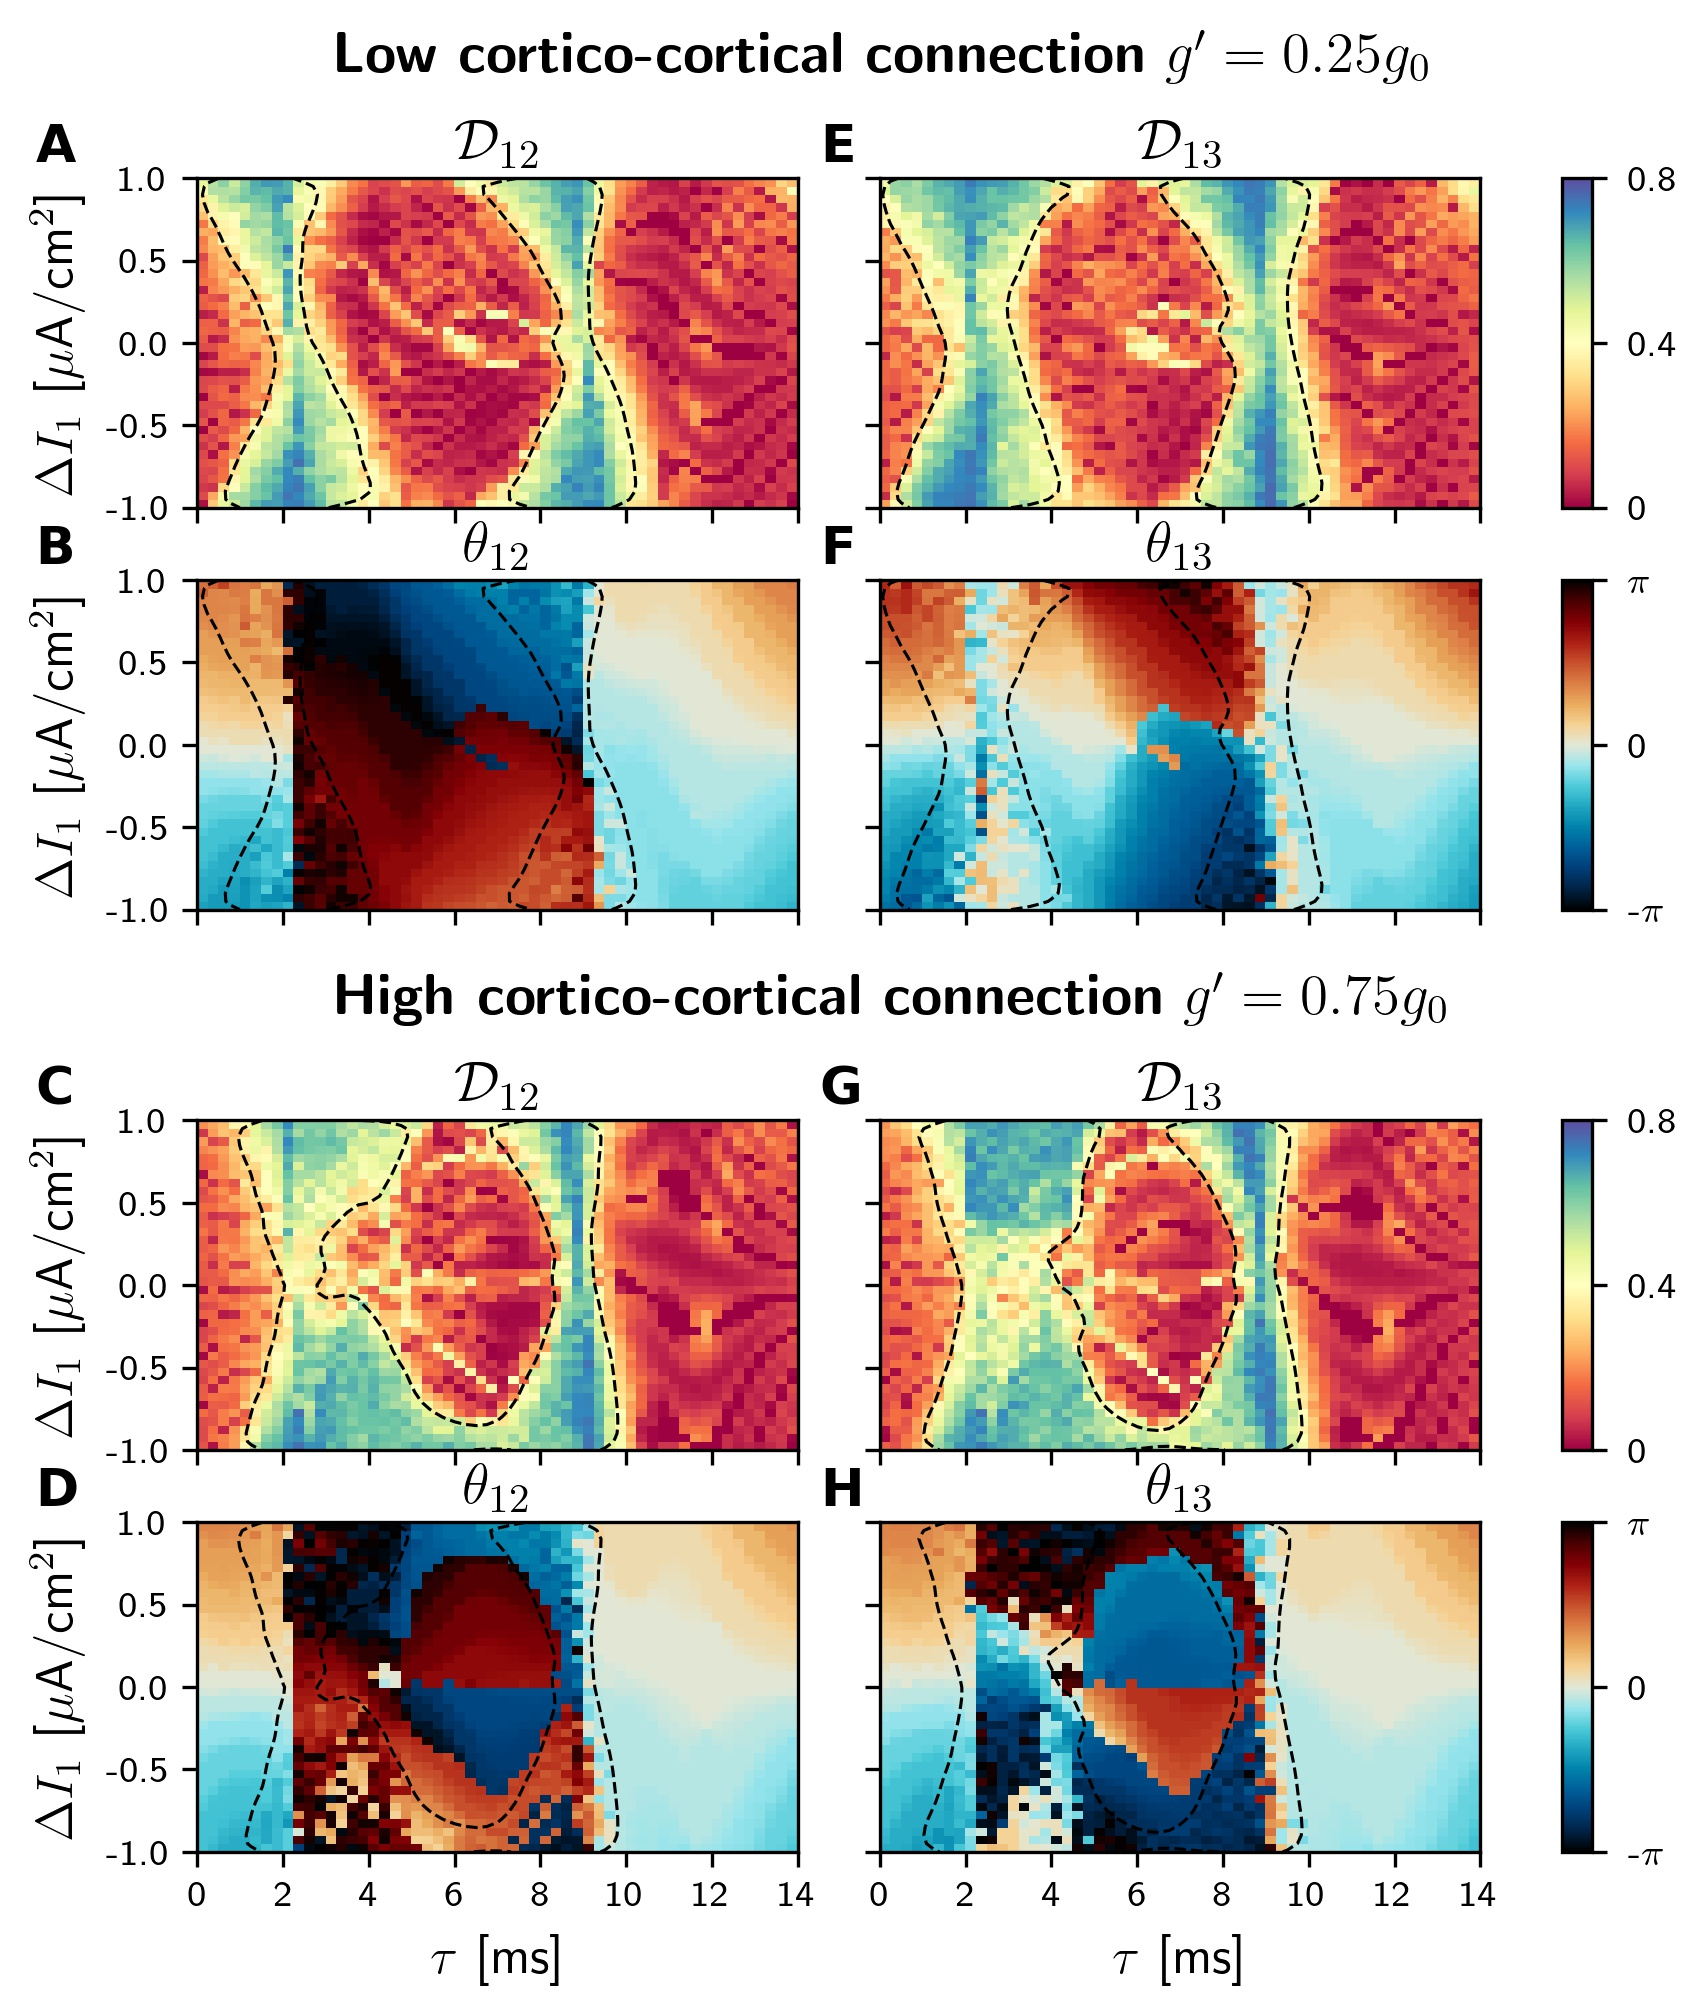
\includegraphics[width=\textwidth]{chapter2/figures/fig5}
    \caption{\textbf{C-motif: phase-locking index and phase difference}.
    Phase-locking index $\mathcal{D}_{ij}$ for $g'=0.25g_0$ (A and E) and $g'=0.75g_0$ (C and G).
    Phase difference $\theta_{ij}$ for $g'=0.25g_0$ (B and F) and $g'=0.75g_0$ (D and H).
    All of them as a function of the delay $\tau$ and the detuning $\Delta I$ in population 1.}
    \label{fig:cmotif_synchro_1}
\end{figure}
Similar to the previous analysis, we examined the distribution of phase differences and the conditions of phase-locking in the parameter space.
\begin{figure}[!htb]
 \centering
    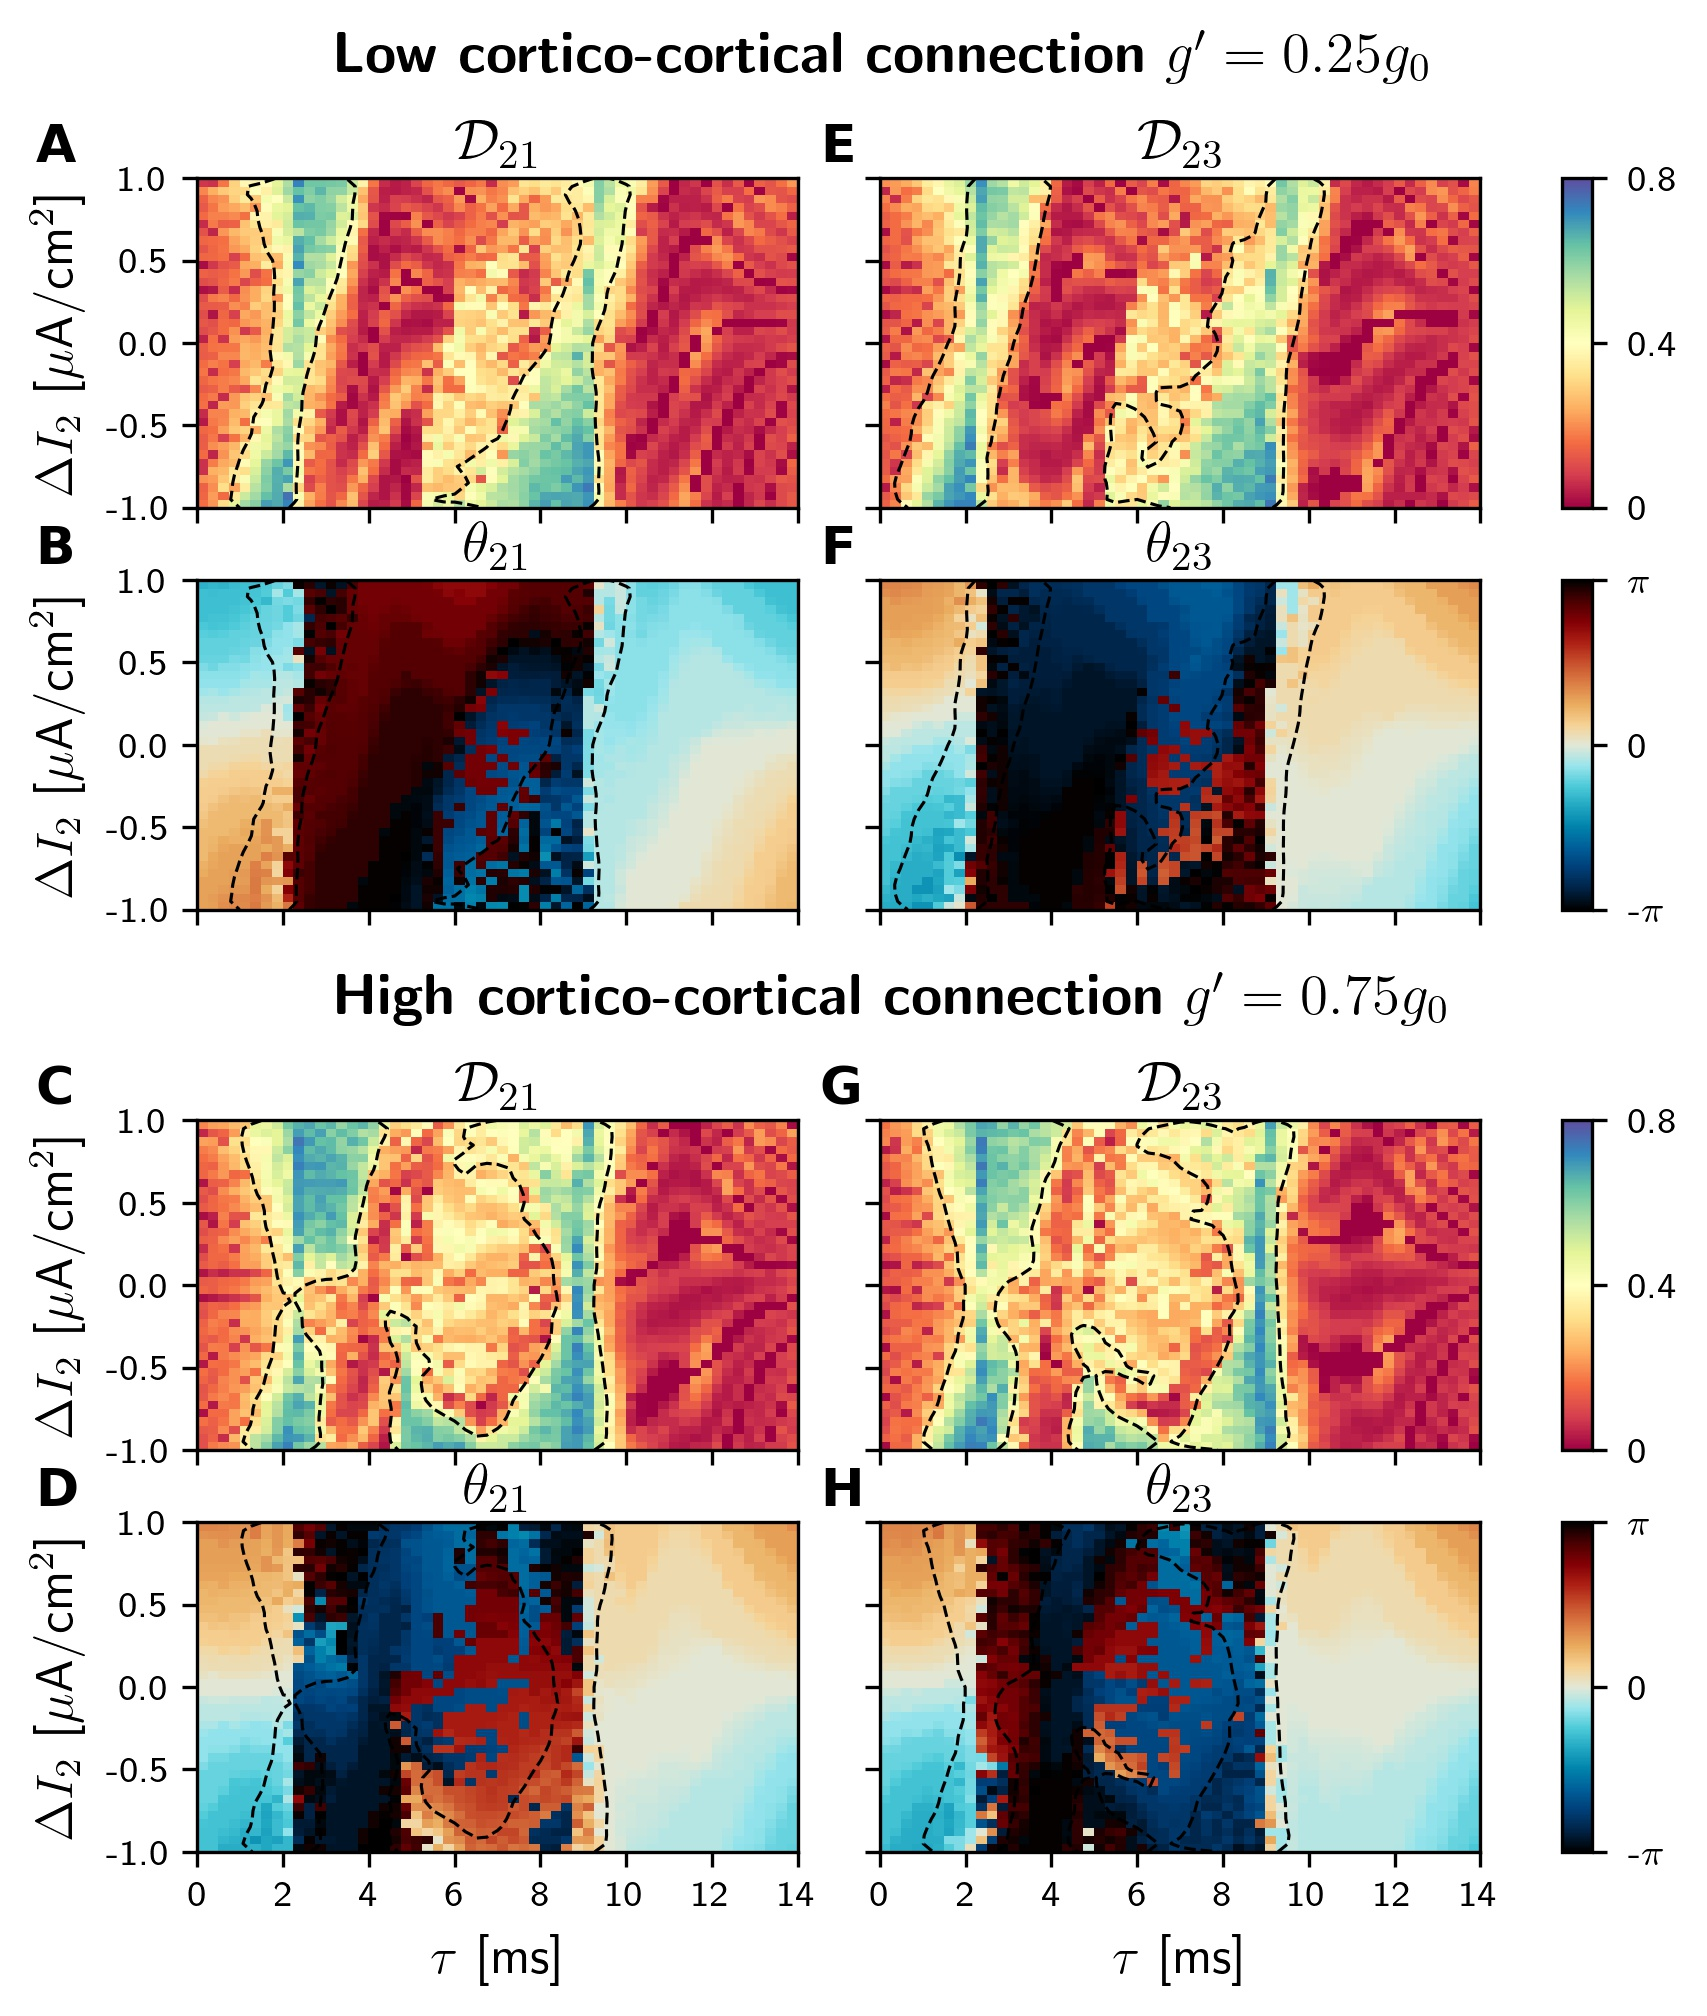
\includegraphics[width=\textwidth]{chapter2/figures/fig7}
    \caption{\textbf{C-motif: phase-locking index and phase differences}.
    Phase-locking index $\mathcal{D}_{ij}$ for $g'=0.25g_0$ (A and E) and $g'=0.75g_0$ (C and G).
    Phase difference $\theta_{ij}$ for $g'=0.25g_0$ (B and F) and $g'=0.75g_0$ (D and H).
    All of them as a function of the delay $\tau$ and the detuning $\Delta I$ in population 2.}
    \label{fig:cmotif_synchro_2}
\end{figure}

Figures \ref{fig:cmotif_synchro_1} and \ref{fig:cmotif_synchro_2} display the phase-locking index and phase differences for low and high values of cortico-cortical synaptic conductance $g'$ when the detuning is applied to populations 1 and 2, respectively (Appendix A, Figures \ref{a-fig:cmotif_locking_1}, \ref{a-fig:cmotif_phase_difference_1}, \ref{a-fig:cmotif_locking_2}, and \ref{a-fig:cmotif_phase_difference_2} for all the different $g'$ values).

Based on the theory of coupled oscillators and our first analysis done with Kuramoto oscillators, in the absence of frequency mismatch, two identical and mutually coupled oscillators with delayed connections can exhibit two synchronization regimes: in-phase and anti-phase (as shown in Figure \ref{fig:2motif-syncrhonization}) \citep{d2008synchronization}.
Consequently, introducing the third connection to our V-motif intensifies the competition between the V-motif dynamics and the dynamics favored by the mutual coupling of the external populations.
While the V-motif structure tends to synchronize populations 1 and 3 at zero-phase (or close to zero-phase) regardless of the connection delay, the additional direct connection between populations 1 and 3 tends to synchronize them in anti-phase at intermediate delay values, giving rise to bistability.

In the circular motif, for small values of the synaptic strength $g'$, the impact of the new connections is minimal, as depicted in panels A, E, and B, F, H of Figure \ref{fig:cmotif_synchro_1}.
However, as $g'$ is increased, its effect becomes noticeable in the phase differences and the size of the locking regions decreases, as shown in panels C, G, and D, H of Figure \ref{fig:cmotif_synchro_1}.
The competition between the V motif's zero (or near-zero) phase-locking and the mutually coupled populations' $\pi$ (or near-$\pi$) phase-locking only occurs within an intermediate range of delay values, as both systems exhibit in-phase dynamics for small and large delay values.
We observed that within this window of delay values, the phase-locking index increased with higher synaptic strength $g'$. % (results not shown).

\subsection{Information transmission in the circular motif}
The competition between the two dynamics mentioned in the previous section has a direct impact on the efficiency of information transmission within the system.
To investigate this further, we examined the propagation of both slow and fast signals with population 1 and population 2 acting as the senders.
Figure \ref{fig:cmotif_signal_1} displays the differences $\Delta$MI$_{ij}$ for slow modulation injected in population 1, with panels A and E representing small $g'$ values and panels C and G representing large $g'$ values (Appendinx A Figure \ref{a-fig:cmotif_dmi_1} for all considered $g'$ values and Figure\ref{a-fig:cmotif_cov_1} for corresponding ZLC results).
Notably, the effect of the cortico-cortical connection becomes noticeable when $g' = 0.75 g_0$.
\begin{figure}[!htb]
 \centering
    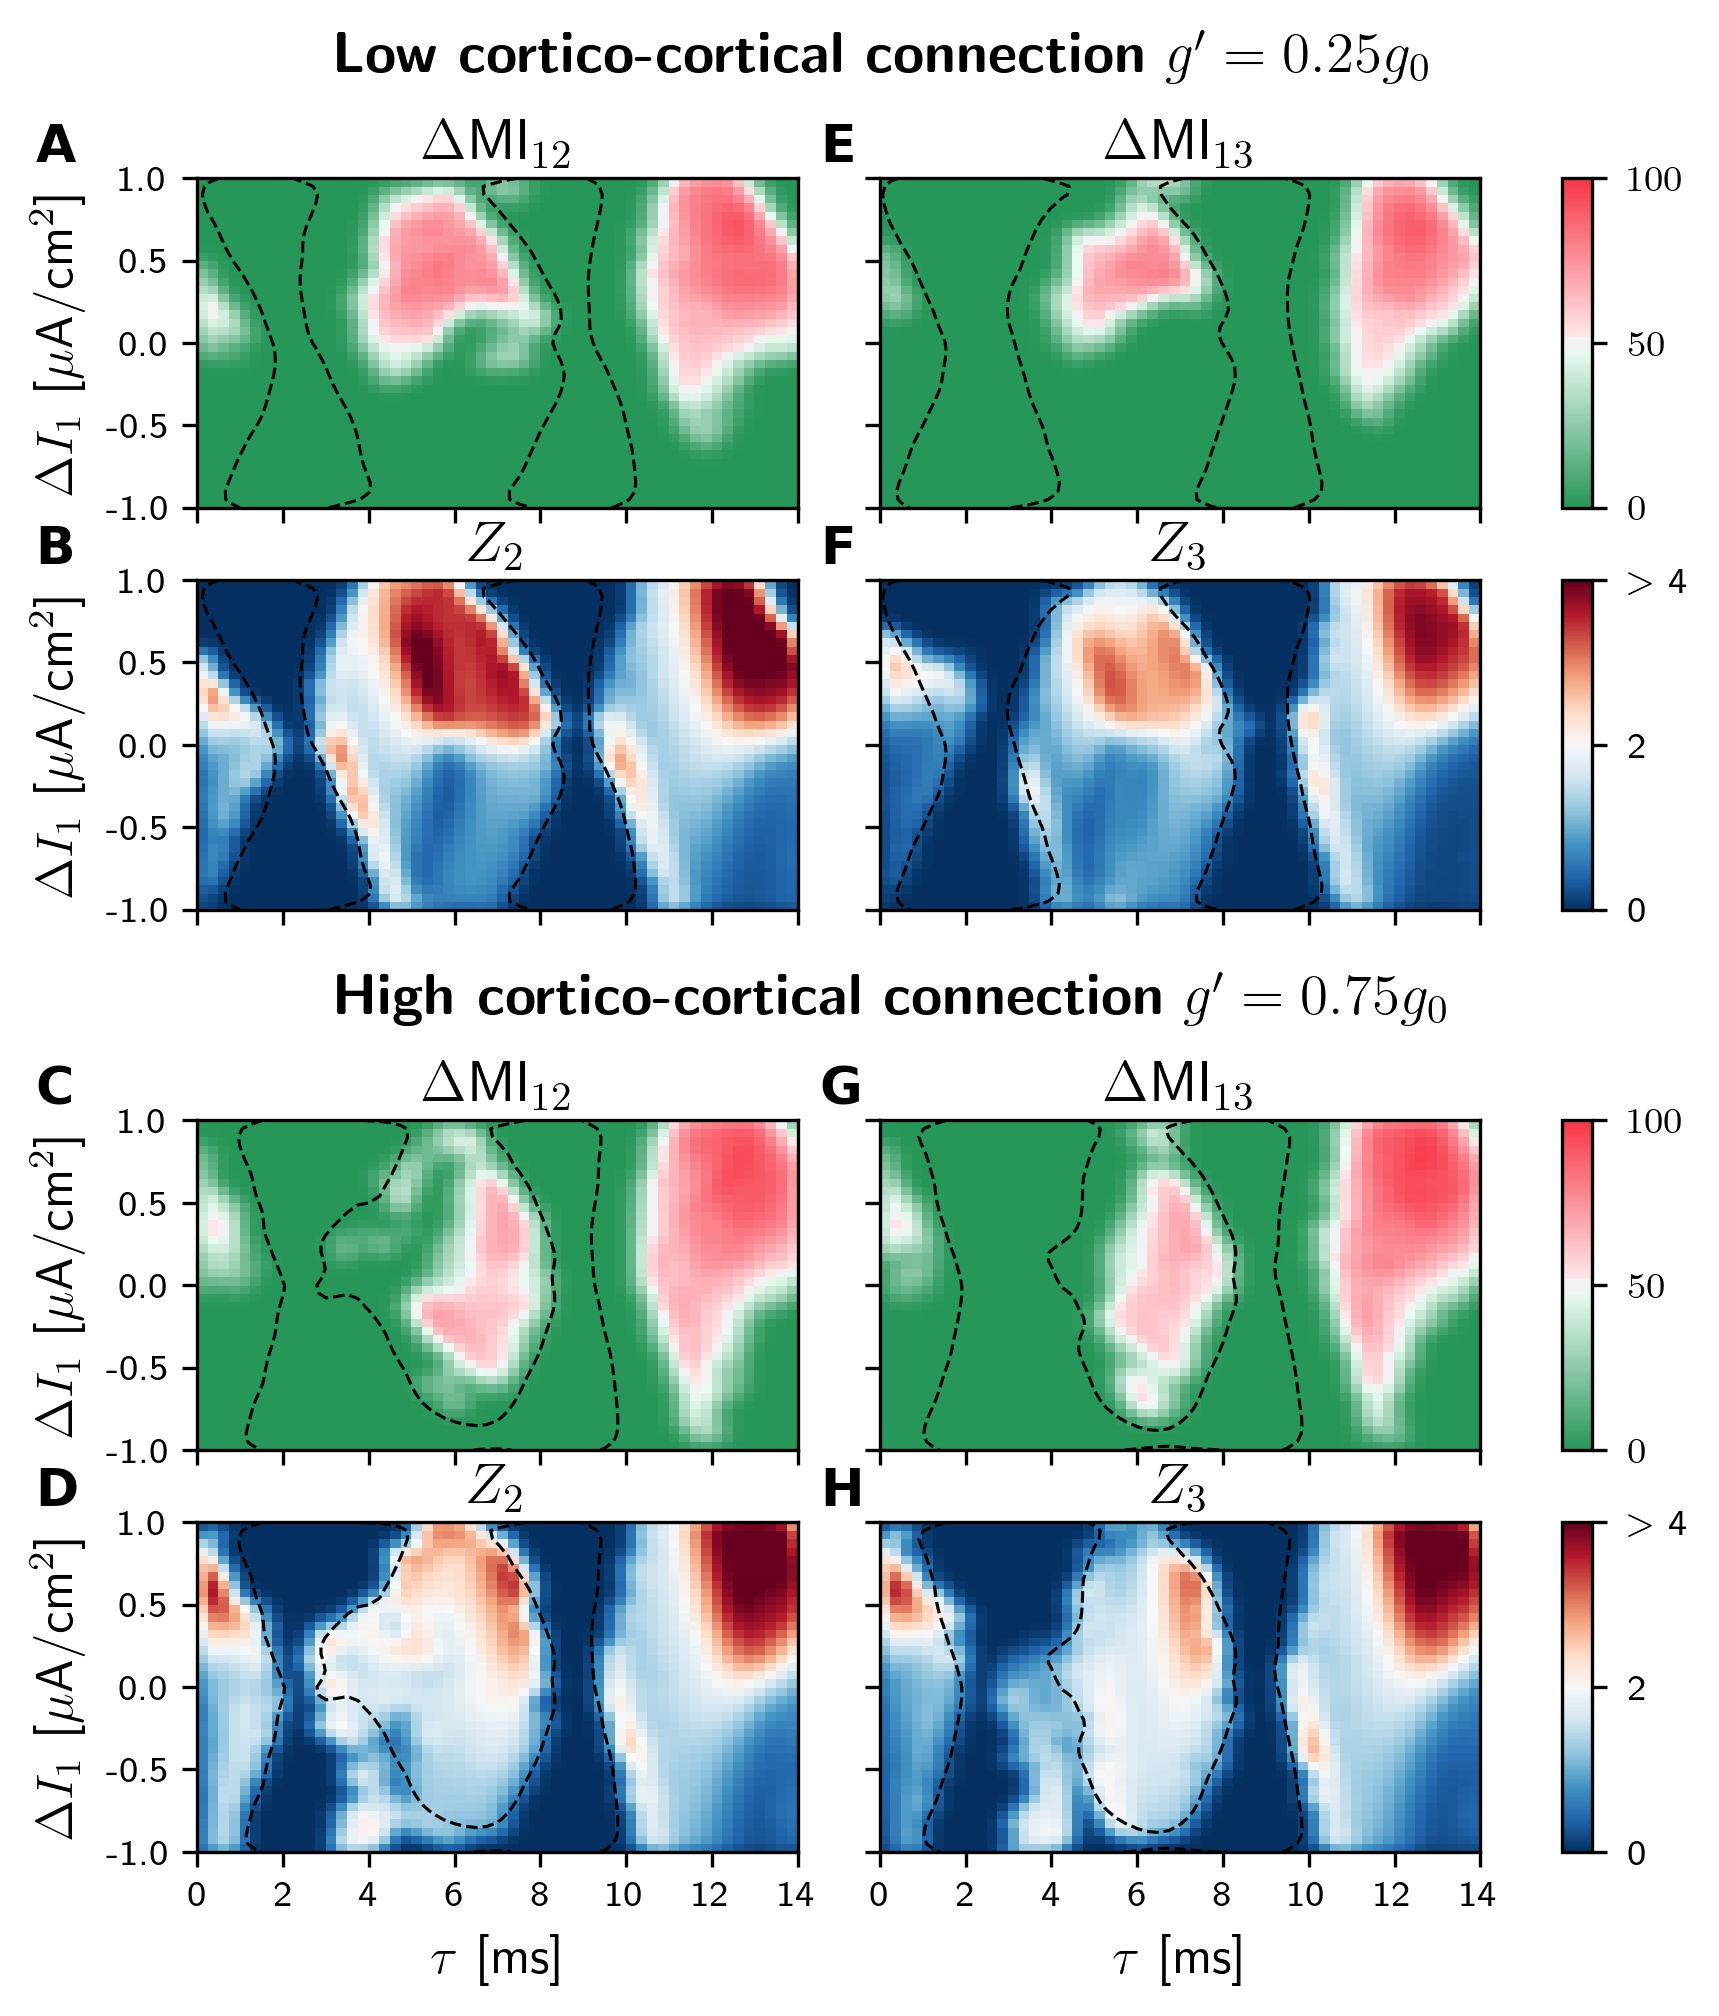
\includegraphics[width=\textwidth]{chapter2/figures/fig6}
    \caption{\textbf{C-motif: population 1 as the sender}.
    Difference $\Delta$MI$_{ij}$ for $g'=0.25g_0$ (A and E) and $g'=0.75g_0$ (C and G).
    Integral of the absolute value of the nPRC $Z_i$ for $g'=0.25g_0$ (B and F) and $g' = 0.75g_0$ (D and H).
    All of them as a function of the delay $\tau$ and the detuning $\Delta I$ in population 1.}
    \label{fig:cmotif_signal_1}
\end{figure}
Comparing this with the case of $g' = 0.25 g_0$, the regions exhibiting good transmission for intermediate delay values change shape, and the values of $\Delta$MI$_{ij}$ (indicating transmission strength and directionality) become smaller.
However, the situation differs from that of the V-motif as the transmission is enhanced for negative detuning (negative values of the current mismatch $\Delta I$) for populations 1 and 2, as well as 1 and 3.
\begin{figure}[!htb]
 \centering
    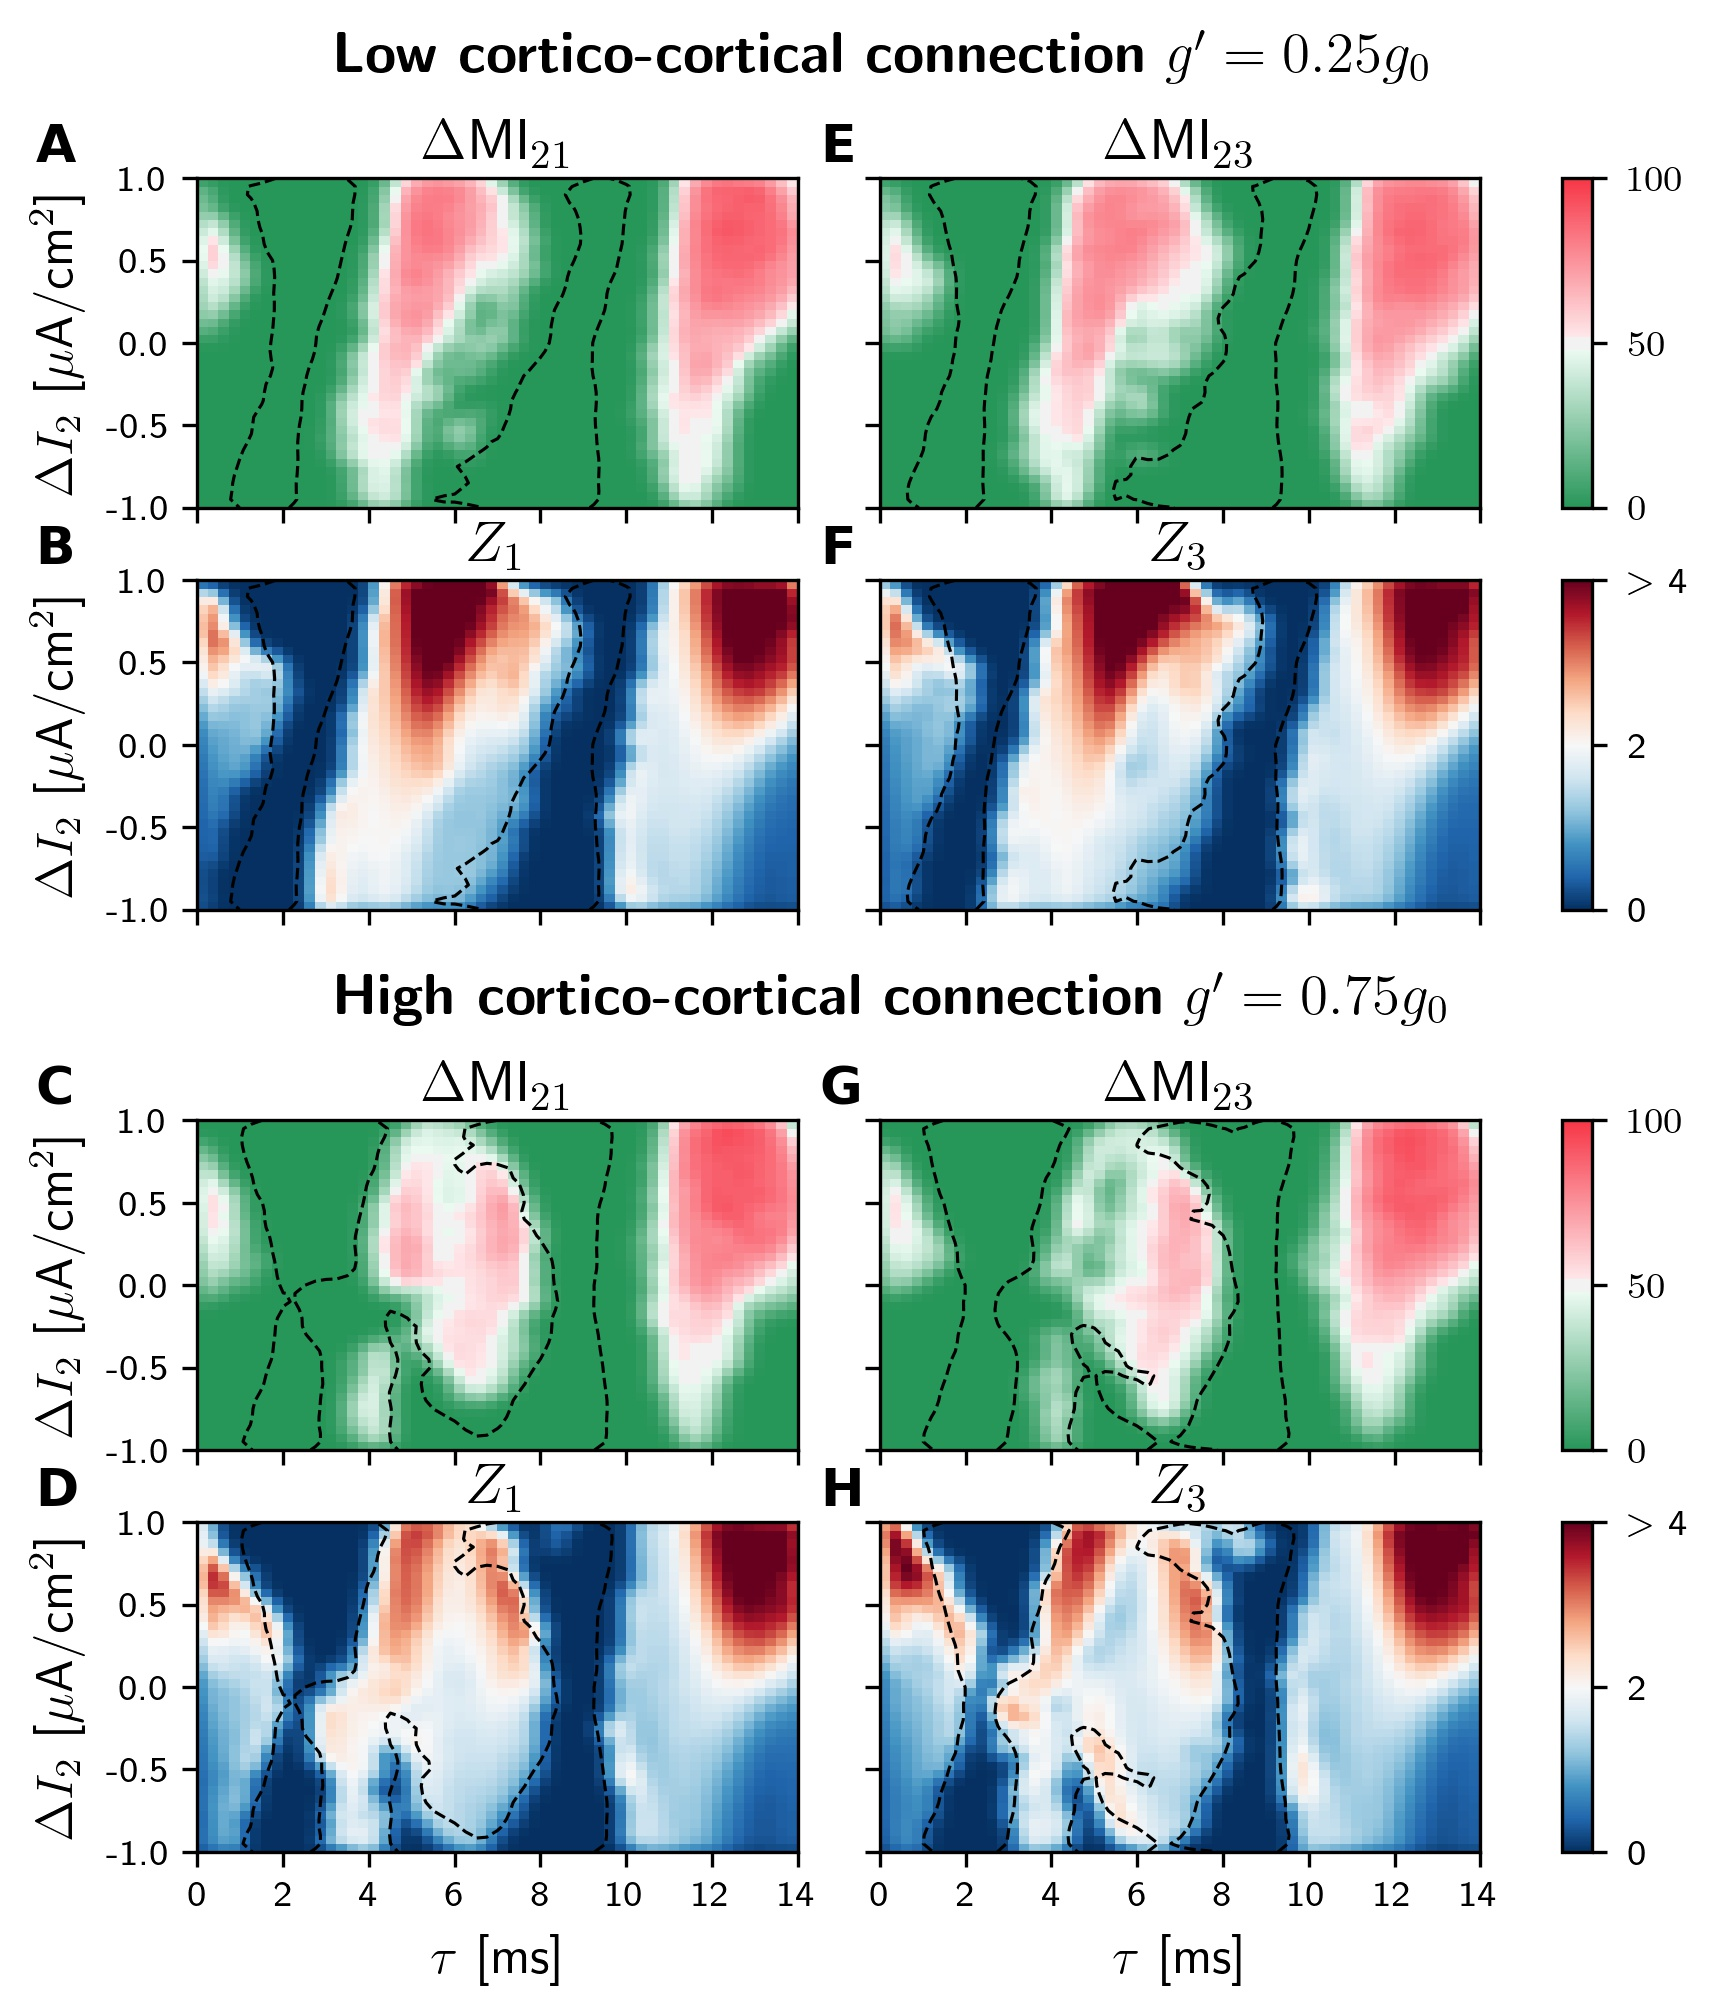
\includegraphics[width=\textwidth]{chapter2/figures/fig8}
    \caption{\textbf{C-motif: population 2 as the sender}.
    Difference $\Delta$MI$_{ij}$ for $g'=0.25g_0$ (A and E) and $g'=0.75g_0$ (C and G).
    Integral of the absolute value of the nPRC $Z_i$ for $g'=0.25g_0$ (B and F) and $g'=0.75g_0$ (D and H).
    All of them as a function of the delay $\tau$ and the detuning $\Delta I$ in population 2.}
    \label{fig:cmotif_signal_2}
\end{figure}
Furthermore, this enhancement is also observed for large delay values.
We also observed that communication for negative detunings improves as the synaptic weight $g'$ increases. % (results not shown).

Similar to the case of slow signals, when injecting a fast pulsating signal, the results are comparable, as shown in Figure \ref{fig:cmotif_signal_1}, with panels B and F representing low $g'$ values and panels D and H representing high $g'$ values.
For $g' = 0.75g_0$ and intermediate delay values, transmission is moderately enhanced for negative detuning, contrasting with the V-motif case.
Moreover, for high delay values, transmission is generally enhanced, but with less significant effects for negative detunings (Appendinx A Figure \ref{a-fig:cmotif_prc_1} for different $g'$ values).

When considering population 2 as the sender population, important changes in the system's behavior occur in the intermediate region, as illustrated in Figure \ref{fig:cmotif_signal_2} (Appendinx A Figure \ref{a-fig:cmotif_prc_2} for different $g'$ values).
Once again, the regions of signal transmission exhibit less dependence on detuning and delay.
Overall, our results indicate that the quality of signal transmission is not significantly influenced by whether the external modulation is slow or fast, regardless of whether it is in the V-motif or in the C-motif.
The crucial factor influencing transmission is the introduction of the cortico-cortical connection between populations 1 and 3.
While this connection diminishes the robustness and efficacy of transmission, it still enables the transfer of information, even in the presence of negative detunings.

\end{document}